\documentclass[onecolumn]{jarticle}
\usepackage{array,booktabs,bytefield}
\usepackage{graphicx, here}
\begin{document}

\pagenumbering{roman}

\title{Enhancement of ALSA firewire stack}
\author{Takashi Sakamoto}
\date{2014/07/23}
\maketitle{}

\begin{abstract}

2000年以降、IEEE 1394バスに接続するサウンドデバイスが発売されている。これらをサポートするために、ALSA - Linuxのサウンドサブシステム - は、カーネルランドにドライバースタックを持っている。だが、このスタックはほんの少数のデバイスをサポートしているに過ぎない。PCM標本を送信することしかできないからだ。これは、音楽制作のためのデバイスにとっては不十分である。こういったデバイスはドライバーに対し、受信パケットのタイムスタンプ処理や、ひとつのパケットへの異なる種類のデータのマルチプレクス/デマルチプレクスを要求するからだ。ALSAの代わりに、FFADO - ユーザーランドドライバ開発プロジェクト - は、たくさんのデバイスをサポートしている。だが、ALSAアプリケーションがFFADOを直接使う方法は提供されていない。2004年に、ALSAのfirewireスタックは拡張され、ALSAのアプリケーションがより多くのデバイスをサポートできるよう、追加で80デバイスをサポートした。この拡張はLinux 3.16にプルされた。

\end{abstract}

\section*{Acknowledgement}

この仕事をするにあたり、私を手助けしてくれた人に感謝します。特に2人の開発者と、3人の献身的なテスターに感謝します。Clemens LadischはALSAのfirewireスタックのメンテナーだ。Fireworksドライバーに対する彼の仕事なしには、私はこのカテゴリーのデバイスに関心を持つことはなかった。更に、彼のコメントやレビューがなしには、私のパッチがALSAの上流にマージされることはなかった。Daniel Wagnerは以前のFreeBoBプロジェクトの創始者だ。彼の手助けなしには、私はBeBoB関連の資料に触れることができなかったし、BeBoBの機能を理解する機会もなかった。Darren Anderson、Maximilian Engelhardt、David Henningssonの3人は、彼らが持っているデバイスを使い、献身的に私のドライバーをテストしてくれた。彼らの継続的なそして意味のあるフィードバックなしには、私は自分の開発したドライバに対する確信を持つことはなかっただろう。

\newpage

\tableofcontents

\newpage

\pagenumbering{arabic}

\section{Introduction}

Linuxは様々なプラットフォームで使われるオペレーティングシステムだ。そのサウンドダブシステム - Advanced Linux Sound Architecture (ALSA) - もまた様々なプラットフォームで使われている。PC/AT互換のプラットフォームにおいて、Linuxを音楽制作用途に使おうとする人がいるが、彼らは、音声信号の内部合成や同期といった機能を持つサウンドデバイスを必要とする。彼らの中には(全員ではないだろうが)、こういった要求を叶えるために、IEEE 1394バスに接続するデバイスを好んで使うものがいる。

しかしALSAはそれ自体、こういったデバイスを扱うには、貧弱なソフトウェアスタックしか持たない。ALSAの代わりに、ユーザーランドドライバ開発プロジェクトが彼らの要求を満足させている。その開発プロジェクトはFFADOという。FFADOはアプリケーションに対してライブラリを提供する。このライブラリはデバイスと通信するためのApplication Programming Interface (API) を持つ。ALSAのアプリケーションの一人比べると、FFADOのアプリケーションの数は少ない。また、ALSAのアプリケーションはFFADOを直接使うことができない。これは、ALSAのアプリケーションはこういったデバイスを直接扱うことができないことを意味する。

私\footnote{著者}は、この問題を2009年に意識した。調査の結果、ALSAのfirewireスタックの拡張がベターな解決策だという結論を得た。この結論と私の仕事を説明するために、この報告を書いた。

この報告ではまず、これらデバイスに関連のある仕様を概観する。次にデバイスの機能を述べる。そしてユーザーランドとカーネルランド双方のソフトウェア実装を調査し、ベターな解決策を模索する。。最後にALSAのfirewireスタックに対する私の仕事を説明する。


\section{共通仕様}

IEEE 1394バスに接続するサウンドデバイスは、IEC 61883-1/6を通信プロトコルとして用いる。このプロトコルの主要な特徴は、音声と音楽情報に関するデータをパケット送信することだ。この章では、デバイスの特徴の理解を助けるために、IEEE 1394、IEEE 1212、IEC 61883-1/6、AV/C command、OHCI 1394を参照する。このレポートの目的は仕様の説明ではないので、ソフトウェアドライバの実装に必要な情報への言及だけにとどめておく。

\subsection{IEEE 1394バス}



IEEE 1394はシリアルバスだ. IEEEは最初の標準を1995年に出版している\cite{ieee1394-1}。 2000年から2006年にかけて、いくつかの補足が追加された\cite{ieee1394-1-a, ieee1394-1-b, ieee1394-1-c}。 2008年にこの標準は改定された\cite{ieee1394-2}。

IEEE 1394バスは物理層、リンク層、トランザクション層、シリアルバス管理から成る。このバスではアイソクロナスとアシンクロナスという2種類の通信が利用可能だ。

\subsubsection{物理層}
IEEE 1394物理層はケーブルとバックプレーンという2種類の環境を定義している。だが、私はバックプレーン環境を見たことがない。ここではケーブル環境に関して述べる。ケーブル環境では、特別なケーブルとコネクターが定義されている。この環境では、ツリー型やスター型など、複数のバストポロジーが利用できる。アービトレーションを伴う半二重通信が使われる。通信では、アービトレーションのためにアナログ信号が使われる。アービトレーションの後で、符号化された信号がデジタルデータ転送に用いられる。


\subsubsection{リンク層}
IEEE 1394リンク層はアイソクロナスサイクルを制御する方法、パケットを転送する方法、パケットを断片化する方法を定めている。


\subsubsection{トランザクション層}
IEEE 1394トランザクション層は、同一のバス上にあるノードをコントロールする方法を定めている。このレイヤはノードのアドレッシングやトランザクションの種類のために、IEEE 1212を参照する。

\subsubsection{シリアルバス管理}
IEEE 1394シリアルバス管理は、バストポロジー、アイソクロナス通信の転送方法と資源を定めている。このレイヤーは他のレイヤーと協調して動作する。

\subsubsection{アイソクロナス通信}
IEEE 1394アイソクロナス通信は、秒間8,000パケット (8.0 kHz) の転送を保証する。通信を開始する際は、バス上にある単独のサイクルマスターがcycle startパケットをブロードキャストする。そして同一バス上にある他のノードは、個別のチャンネル番号を持つパケットを転送する。このチャンネルは6ビットフィールドで表現される。受信ノードはチャンネルを用いて受信するパケットを特定する。

\begin{figure}[H]
\centering
\begin{bytefield}[bitwidth=auto,endianness=big]{32}
	\bitheader{0-31} \\
	\begin{rightwordgroup}{packet \\ header}
		\bitbox{16}{data length} &
		\bitbox{2}{tag} &
		\bitbox{6}{channel} &
		\bitbox{4}{tcode} &
		\bitbox{4}{sy} \\
		\wordbox{1}{header CRC}
	\end{rightwordgroup} \\
	\begin{rightwordgroup}{packet payload}
		\wordbox[tlr]{3}{data field} \\
		\bitbox[blr]{16}{} &
		\bitbox{16}{zero pad bytes (if necessary)} \\
		\wordbox{1}{payload CRC}
	\end{rightwordgroup}
\end{bytefield}
\caption{アイソクロナスパケット内容}
\label{fig:iso-packet}
\end{figure}

In Figure \ref{fig:iso-packet}, data length: the length of data field, tag: the packet format, channel: the channel number for this packet, tcode: the data format of isochronous packet, sy: application specific control field.

通常、tcodeフィールドの値はb1010。Common Isochronous Packet (CIP) のtagフィールドの値はb01だ\cite{iec61883-1-3}。

\subsubsection{アシンクロナス通信}
IEEE 1394アシンクロナス通信は遅延に対する保証を持たない。パケットは断片化することがある。IEEE 1394トランザクション層がこの通信を処理する。この通信にはquadletとblockという2種類が存在する。

\begin{figure}[H]
\centering
\begin{bytefield}[bitwidth=auto,endianness=big]{32}
	\bitheader{0-31} \\
	\begin{rightwordgroup}{packet \\ header}
		\bitbox{16}{destination ID} &
		\bitbox{6}{tl} &
		\bitbox{2}{rt} &
		\bitbox{4}{\tiny tcode \\ 0000} &
		\bitbox{4}{pri} \\
		\bitbox{16}{source ID} &
		\bitbox[tlr]{16}{destination offset} \\
		\wordbox[blr]{1}{} \\
		\wordbox{1}{quadlet data} \\
		\wordbox{1}{header CRC}
	\end{rightwordgroup} \\
\end{bytefield}
\caption{quadletトランザクションのアシンクロナスパケット内容}
\label{fig:async-packet-quadlet}
\end{figure}

\begin{figure}[H]
\centering
\begin{bytefield}[bitwidth=auto,endianness=big]{32}
	\bitheader{0-31} \\
	\begin{rightwordgroup}{packet \\ header}
		\bitbox{16}{destination ID} &
		\bitbox{6}{tl} &
		\bitbox{2}{rt} &
		\bitbox{4}{\tiny tcode \\ 0001} &
		\bitbox{4}{pri} \\
		\bitbox{16}{source ID} &
		\bitbox[tlr]{16}{destination offset} \\
		\wordbox[blr]{1}{} \\
		\bitbox{16}{data length} &
		\bitbox{16}{extended code} \\
		\wordbox{1}{header CRC} 
	\end{rightwordgroup} \\
	\begin{rightwordgroup}{payload}
		\wordbox[tlr]{3}{block data} \\
		\bitbox[blr]{16}{} &
		\bitbox{16}{zero pad bytes (if necessary)} \\
		\wordbox{1}{payload CRC}
	\end{rightwordgroup}
\end{bytefield}
\caption{blockトランザクションのアシンクロナスパケット内容}
\label{fig:async-packet-block}
\end{figure}

In Figure \ref{fig:async-packet-quadlet} and \ref{fig:async-packet-block}, destination ID: node ID of destination, tl: transaction label for a pair of request and response, rt: the way to retry, tcode: the type of transaction, read/write/lock and quadlet/block and request/response, pri: priority, source ID: node ID of source, destination offset: an address offset on destination's area, data length: the length of byte of block data, extended code: the type of lock transaction.

\subsection{IEEE 1212}

IEEE 1212は、それぞれのデバイスを指す論理アドレス空間とトランザクションの種類の仕様だ。最初の版は1991年に出版され\cite{ieee1212-1}、ISO/IEC 13213\cite{iso13213}で標準化された。第2版は2001年に出版され、第1版を置きかえた。

IEEE 1212はmodule、node、unitというバス上のエンティティーを定める。moduleは複数のnodeを含み、nodeは複数のunitを含む。nodeは64ビットの値でアドレスされる。このアドレスを含むトランザクションにより、ノード間通信を行う。IEEE 1212はread、write、lockという3種類のトランザクションを定める。各ノードのアドレス空間はノードの状態を制御するために、Control and Status Registers (CSR) を持つ。アドレス空間は、ノードとユニットの情報を示すために、Configuration ROMを持つ。


\subsection{IEC 61883-1}

IEC 61883-1は音声映像データ通信プロトコルと、デジタルオーディオビデオ装置同士の相互接続を制御するコマンドを定める。最初の版は1998年に出版された\cite{iec61883-1-1}。第2版は2003年に出版された\cite{iec61883-1-2}。第3版は2008年に出版され、以前の版を置きかえた\cite{iec61883-1-3}。

IEC 61883-1はIEEE 1394バス上のリアルタイムデータ転送プロトコルとCommon Isochronous Packet (CIP)を定める。Common Isochronous Packet は IEEE 1394アイソクロナスパケットのペイロードの標準データフォーマットだ。CIP の詳細は次の節で述べる。

このデータ転送はコネクションという概念で制御される。コネクションは、Plug Control Register (PCR) で表現される。Master Plug Register (MPR) は PCR の基本情報を持つ。MPRとPCRのどちらも32ビットレジスターだ。レジスターは0xFFFF'F000'0900から0xFFFF'F000'09FCにある。この領域の最初の半分は出力プラグ用で、残りは入力プラグ用だ。それぞれの領域の最初の32ビットレジスターがMPRとなる。


コネクションはConnection Management Procedure (CMP) で制御される。CMPにおいては、lockトランザクションを用いてPCRのフィールド変更し、コネクションの確立と切断を行う。

それぞれのnodeの機能は Function Control Protocol (FCP) で制御される。FCPはコマンドとレスポンスというトランザクションのペアから成る。コマンドの送られるアドレスは0xFFFF'F000'0B00で、レスポンスの送られるアドレスは0xFFFF'F000'0D00だ。トランザクション長は512バイトに限定されている。


\subsection{IEC 61883-6}

IEC 61883-6はオーディオとミュージック情報に対するIEC 61883-1の派生だ。AMDTPとも呼ばれる。最初の版は2002年に出版された\cite{iec61883-6-1}。第2版はたくさんの拡張と共に、2005年に出版された\cite{iec61883-6-2}。

IEC 61883-1\cite{iec61883-1-1, iec61883-1-2, iec61883-1-3}はCIP構造の派生を許可している。CIPヘッダはいくつかの32ビットフィールドから成る。MSBの最初のビットはEnd-of-CIP-header (EOH) だ。このビットは最後のCIPヘッダで立つ。MSBの2番目のビットは Form だ。このビットは続くフィールドの種類を示すようだが、その意味については曖昧でよくわからない。AMDTPにおいては、SYTフィールドを含む2つのCIPヘッダが使われる。図\ref{fig:amdtp-cip}にCIP内容を示す。マイナーなフィールドは0で示す。

\begin{figure}[H]
\centering
\begin{bytefield}[bitwidth=auto,endianness=big]{32}
	\bitheader{0-31} \\
	\begin{rightwordgroup}{CIP header \\ with SYT field}
		\bitbox{1}{0} &
		\bitbox{1}{0} &
		\bitbox{6}{SID} &
		\bitbox{8}{DBS} &
		\bitbox{2}{00} &
		\bitbox{3}{000} &
		\bitbox{1}{0} &
		\bitbox{2}{000} &
		\bitbox{8}{DBC} \\
		\bitbox{1}{1} &
		\bitbox{1}{0} &
		\bitbox{6}{FMT} &
		\bitbox{8}{FDF} &
		\bitbox{16}{SYT}
	\end{rightwordgroup} \\
	\begin{rightwordgroup}{data block \\ = event 1}
		\wordbox[tlr]{1}{data} \\
		\wordbox[blr]{1}{$\cdots$}
	\end{rightwordgroup} \\
	\begin{rightwordgroup}{data block \\ = event 2}
		\wordbox[tlr]{1}{data} \\
		\wordbox[blr]{1}{$\cdots$}
	\end{rightwordgroup} \\
	\wordbox{1}{$\cdots$} \\
\end{bytefield}
\caption{AMDTP用のCIP派生}
\label{fig:amdtp-cip}
\end{figure}

In Figure \ref{fig:amdtp-cip}, SID: the node ID of transmitter, DBS: the number of quadlets for data blocks, DBC: the number of data blocks which has already transferred, FMT: format ID, FDF: format dependent field, SYT: the offset from isochronous cycle timer.

DBCフィールドの値は、パケット喪失を検出するために用いられる。AMDTPにおいては、FMTの値は0x10、FDFは後述する Event TypeフィールドとSampling Frequency Codeフィールドから成る。一方で、データを持たないパケットを示すために、FDFフィールドには0x00も使われる。AMDTPにおいては、SYTフィールドの値はpresentation timeを示すために用いられる。詳細は\pageref{sec:clock-recovery}ページの\ref{sec:clock-recovery}章で述べる。


データブロックがCIPヘッダーに続く。AMDTPにおいては、ひとつのデータブロックがひとつのeventを示す。IEC 61883-6\cite{iec61883-6-1, iec61883-6-2} はeventの意味を定めていないが、同一のタイミングを持つデータの集合だと思う。データの表現方法がいくつかあり、AM824がよく用いられる。

AM824はデータを32ビットフィールドで表現する。32ビットのうち、8ビットがラベルに使われ、24ビットがデータに使われる。IEC 61883-6:2002\cite{iec61883-6-1}では、AM824は3種類のデータを記述できる。すなわち、IEC 60958 Conformant、Raw Audio、MIDI Conformantである。IEC 61883-6:2005\cite{iec61883-6-2}では、Raw AudioはMulti Bit Linear Audio (MBLA) に名前が変わり、新しいデータタイプが追加された。

eventは音声と音楽のためのもので、AMDTPは標本化周波数に支配される。CIPヘッダのFDFフィールドが標本化周波数とeventの種類を示す。EVTフィールドのMSB側の4ビットがeventデータの記述方法を示し、LSB側の4ビットのうち後半3ビットがSFCフィールドとしてnominal sampling frequencyを示す。残りの1ビットはN-flagで、rateコントロールに使われる。このビットが立っていない場合、\pageref{sec:clock-recovery}ページの\ref{sec:clock-recovery}章に記述しているclock based rateコントロールが用いられる。もし断っている場合、command based rateコントロールが用いられる\cite{iec61883-6-2, avc-rate-control}。AM824においては、EVTフィールドの値はb0000だ。SFCフィールドの値を表\ref{tbl:sfc-fdf}に示す。大抵のサウンドデバイスにおいて、N-flagは立っていない。

\begin{figure}[H]
\centering
\begin{bytefield}[bitwidth=auto,endianness=big]{8}
	\bitheader{0-7} \\
	\bitbox{4}{EVT} &
	\bitbox{1}{N} &
	\bitbox{3}{SFC} &
\end{bytefield}
\caption{FDF field for AMDTP}
\label{amdtp-fdf}
\end{figure}

\begin{table}[H]
	\centering
	\caption{{The value of SFC field in FDF field}}
	\label{tbl:sfc-fdf}
	\begin{tabular}{ccc} \toprule
		Nominal Sampling Frequency & SFC \\ \midrule
		32.0	& b000 \\
		44.1	& b001 \\
		48.0	& b010 \\
		88.2	& b011 \\
		96.0	& b100 \\
		176.4	& b101 \\
		192.0	& b110 \\ \bottomrule
	\end{tabular}
\end{table}

パケット転送方法の詳細に関しては、\pageref{sec:clock-recovery}ページの\ref{sec:clock-recovery}を参照のこと。

\subsection{AV/C コマンド}

IEC 61883シリーズはもともと、1394 Trade Association (1394TA)の出版物に基づいている。特に、FCPの実際のアプリケーションは、1394TAの文書によるしかなく、公開されている文書はない。1394TAの文書においては、FCPのアプリケーションはAV/Cコマンドと呼ばれている。AV/Cコマンドには大量の派生があり、過剰仕様となっている。その一部の仕様が、サウンドデバイスに適用されている\cite{avc-general-4-2, avc-audio-1, avc-connection-1, avc-music-1, avc-descriptor-1, avc-info-block-1, avc-general-enhancement, avc-stream-format-1, avc-stream-format-1-1, avc-rate-control}。

\subsection{1394 Open Host Controller Interface}
\label{ohci-1394}

1394 Open Host Controller Interface (OHCI 1394) は IEEE 1394 リンク層プロトコルの実装だが、トランザクション層やバス管理層を助けるための追加機能も持つ。この仕様は、高パフォーマンスデータ転送とホストバスインターフェイスのために、Direct Media Access (DMA) エンジンを用いる。最初の版は1997年に出版され\cite{ohci1394-1}、2000年に改定された\cite{ohci1394-1-1}。

OHCI 1394はPC/AT互換プラットフォームに対し、レジスター、割り込み、DMAを伴うソフトウェアインターフェイスを記述している。OHCI 1394はPCI/PCI-Expressバス上のカードデバイスとして実装される。

OHCI 1394はアシンクロナスとアイソクロナス通信をコンテキストとして表現する。コンテキストはディスクリプターのリストを含む。このディスクリプターはそれぞれの通信パケットの情報を含む。この情報はDMAバッファーのアドレスを含む。このアドレスによってデータを指し、DMAを用いてデータをシステムとコントローラーデバイス間で転送する。データの転送後、ディスクリプタの情報に合わせて割り込みが発生する。一方向に対し、アイソクロナスコンテキストの最小数は4で、最大数は32となっている。


\section{デバイスの特徴}

音楽制作に使われるサウンドデバイスは固有の機能を持つ。この章では、ソフトウェア実装を考えるために、それら機能を記述する。

\subsection{クロックリカバリー}
\label{sec:clock-recovery}

クロックリカバリーは受信者が、送信者のクロックサイクルを再現するための仕組みだ。

IEEE 1394\cite{ieee1394-2}において、isochronous-capableノードは32ビットのCYCLE\_TIMERレジスターを持たなければならない。このレジスターのLSB側12ビットは、3,072を法とするカウンターで、24.576 MHz (あるいは40.69ナノ秒)毎に1増加する。その上の13ビットは8.0 kHz (あるいは125マイクロ秒) サイクルのカウンターだ。MSB側7ビットは秒のカウンターだ。


\begin{figure}[htbp]
\centering
\begin{bytefield}[bitwidth=auto,endianness=big]{32}
	\bitheader{0-31} \\
	\bitbox{7}{seconds\_count} &
	\bitbox{13}{cycle\_count} &
	\bitbox{12}{cycle\_offset}
\end{bytefield}
\caption{{CYCLE\_TIMERレジスター}}
\label{cycle_timer}
\end{figure}

通常の実装では、このレジスターはIEEE 1394リンク層チップセットが与える24.576 MHzのクロックにしたがってカウントアップする。

cycle\_offsetフィールドがロールオーバーした時、cycle masterノードはアービトレーションを行い、cycle-startパケットをブロードキャストする。このパケットはcycle\_timeフィルドを持ち、このフィールドはCYCLE\_TIMERレジスターの値を持つ。cycle-startパケットを受信すると、アイソクロナスパケットの送信者と受信者は自身のCYCLE\_TIMERレジスターを更新する。結果、アイソクロナスパケットの送信者と受信者はローカルに、cycle masterノードに対する時間リファレンスを持つことになる。そして、アイソクロナスパケットの送信者はアービトレーションを開始し、その後アイソクロナスパケットを特定のチャンネルに向けて送信する。受信者は好みのチャンネルのアイソクロナスパケットを受信する。各cycle-startパケットの実際のインターバルは、バスのバンド幅使用率によって変化する。図\ref{fig:cycle-start}を参照のこと。


\begin{figure}[htbp]
\centering

\includegraphics[scale=0.75]{./img/cycle-start-packet.svg.eps}
\caption{{cycle-startパケットとnominal isochronous cycle}}
\label{fig:cycle-start}
\end{figure}

IEC 61883-1はCIPヘッダにSYTフィールドを定めている (\pageref{fig:amdtp-cip}ページの図\ref{fig:amdtp-cip}を見よ)。IEC 61883-6では、このフィールドを使ってpresentation timeを計算する。presentation timeはパケット内の特定のイベントのタイムスタンプを表現する。送信者は先程のローカルな時間リファレンスから標本化クロックのオフセットを計算し、SYTフィールドに入れてパケットを送信する。受信者はパケットのSYTフィールドとローカルの時間リファレンスからpresentation timeを計算する。

一つのパケットのCIPヘッダにはひとつのSYTフィールドしかない。一方で一つのパケットはいくつかのデータブロックを持つ。そのため全てのデータブロックがpresentation timeを持つことができない。そこで、presentation timeを伴うデータブロックのインターバルがSYT\_INTERVALとして定められている。


One packet has one SYT field in its CIP header, while one packet can include several data blocks. All of data blocks cannot have 'presentation time'. The interval between data blocks with 'presentation time' is defined as SYT\_INTERVAL.

\begin{table}[ht]
	\centering
	\caption{{SYT\_INTERVALの値}}
	\label{syt_interval}
	\begin{tabular}{cc} \toprule
		Sample transmission frequency & SYT\_INTERVAL \\ \midrule
		32.0	& 8	\\
		44.1	& 8	\\
		48.0	& 8	\\
		88.2	& 16	\\
		96.0	& 16	\\
		176.4	& 32	\\
		192.0	& 32	\\ \bottomrule
	\end{tabular}
\end{table}

もしpresentation timeを伴うデータブロックをパケットが含まなければ、SYTの値はNo Informationコード (0xffff) となる。presentation timeを伴うデータブロックの決定方法は、パケット転送モードによって異なる。

IEC 61883-6\cite{iec61883-6-1,iec61883-6-2}においては、2つのパケット転送モードが定められている。ひとつはblocking、もうひとつはnon-blockingだ。これら2つのモードの違いは、転送遅延と、ひとつのパケットが含むデータブロックの数だ。

blockingモードでは、ひとつのパケットが含むデータブロックの数はSYT\_INTERVALと同じ数に固定されている。従ってpresentation timeはパケットの最初のデータブロックのものになる。転送者はパケットに含まれる全ての標本が標本化されるまで待たなければならないため、転送遅延はデフォルト値よりもパケットひとつぶん大きくなる。


\begin{figure}[H]
	\centering
	
\includegraphics[scale=0.6]{./img/amdtp-blocking.svg.eps}
	\caption{{blockingモードのAMDTP}}
	\label{amdtp-blocking}
\end{figure}

non-blockingモードでは、ひとつのパケットは異なる数のデータブロックを含むことができる。転送者はパケットが含む全ての標本が標本化されるのを待たずに、nominal isochronous cycleに従ってパケットを転送する。転送遅延はデフォルト値のままだが、パケット内のどのデータブロックがpresentation timeを伴うかを決定する方法はより複雑となる。

\begin{figure}[H]
	\centering
	\includegraphics[scale=0.6]{./img/amdtp-nonblocking.svg.eps}
	\caption{{non-blockingモードのAMDTP}}
	\label{amdtp-nonblockingstart}
\end{figure}

転送者はpresentation timeを伴うデータブロックを、以下の条件で決定する:

\begin{equation}
	mod(DBC, SYT\_INTERVAL) = 0
\end{equation}

受信者はpresentation timeを伴うデータブロックのインデックスを以下の式で決定する:

\begin{equation}
	index = mod((SYT\_INTERVAL - mod(DBC, SYT\_INTERVAL)), SYT\_INTERVAL)
\end{equation}

どちらのモードにおいても、受信者はSYTフィールドの値とローカルな時間リファレンスから、synchronization clock frequencyを生成する。この時、以下の式が使われる。

\begin{equation}
	Fsync = STF / SYT\_INTERVAL < 8,000
\end{equation}

ここで、Fsyncはsynchronization clock frequencyのことである。STFはsampling transmission frequencyを示し、sampling clock frequencyと同値である。

\begin{table}[H]
	\centering
	\caption{{それぞれのsampling transmission frequencyにおけるSynchronization clock frequency}}
	\label{fsync}
	\begin{tabular}{ccc} \toprule
		STF & SYT\_INTERVAL & Fsync \\ \midrule
		32.0	& 8	& 4,000 \\
		44.1	& 8	& 5,512 \\
		48.0	& 8	& 6,000 \\
		88.2	& 16	& 5,512 \\
		96.0	& 16	& 6,000 \\
		176.4	& 32	& 5,512 \\
		192.0	& 32	& 6,000 \\ \bottomrule
	\end{tabular}
\end{table}

受信者はこの周波数のパルスをPhase Lock Loop (PLL) 回路のリファレンスとして使うことができる。これが、クロックリカバリーと呼ばれる仕組みである。実際の実装に関する例は、\cite{icelynx}を参照のこと。



\subsection{内部ミックスのための信号処理}
\label{sec:internal-mixing}

音楽制作のためのほとんどのデバイスは、アナログ/デジタル音声入出力のためのポートをいくつか持つ。そういったデバイスはポート間の信号をDSPで処理して、内部ミックスを行う。ハードウェアベンダーはこれを、zero latency hardware monitoringと呼んでいる。

DSPの視点に立つと、デバイスが出力するアイソクロナスパケットは音声信号のsinkにあたり、入力パケットは音声信号のsourceにあたる。DSPはIEC 61883-1/6層とDAC/ADCの間にあるため、sinkとsourceをつなぐ設置をDSPが持たない場合は、デバイスは音声を生成しないことになる。

DSPの挙動を制御する方法は、それぞれのデバイスチップセットやモデルによって異なる。

\begin{figure}[H]
	\centering
	
\includegraphics{./img/dsp-route.svg.eps}
	\caption{{sourceとsinkの間の信号処理}}
	\label{dsp-route}
\end{figure}

\subsection{DSPの標本化クロック源に対するオプション}

音楽制作用途に使われる大抵のデバイスは、クロック源に対していくつかのオプションを持つ。このクロック源はDSPの入力クロックとして用いられる。オプションは:
\begin{itemize}
	\item 内部クロック源からの信号
	\item S/PDIF、ADAT、Word Clockからの入力信号
	\item nominal isochronous cycleの信号 (8kHz)
	\item 前節で言及したクロックリカバリーの信号 (4.0/5.512/6.0kHz)
\end{itemize}

現在のクロック源を変更する方法は、それぞれのデバイスチップセットにより異なる。外部クロック源が選択されている時、標本化周波数はそのクロックからの信号に従って固定されなければならない。


\subsection{タイムスタンプ同期する双方向ストリーム}
\label{sec:duplex-streams}

前節で述べたとおり、それぞれのAMDTPパケットはSYTフィールドの値の連続としてpresentation timeを配ぶ。2つのデバイスが双方向ストリームをサポートしている場合、最適な同期のためには、タイムスタンプの生成側は転送側と送信側のうち、どちらか1つでなければならない。この理想はタイミングスレーブ側に対し、受信パケットのSYTフィールド値を用いて送信パケットのSYTフィールドの値を再生成することを要求する。


\begin{figure}[H]
	\centering
	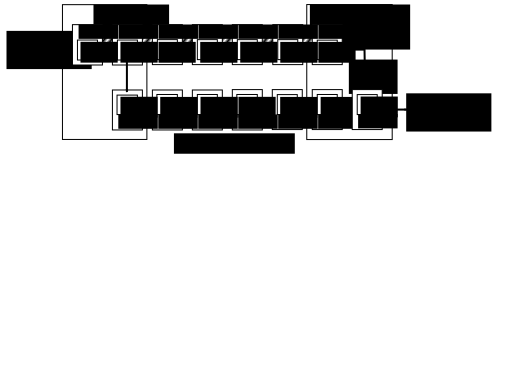
\includegraphics{./img/duplex-timestamp.svg.eps}
	\caption{{双方向ストリーム、タイミングマスターおよびスレーブ}}
	\label{duplex-timestamp}
\end{figure}


\subsection{パケットのデータブロックにおける異なるデータチャンネル構成}
\label{sec:formation-data-block}

IEC 61883-6\cite{iec61883-6-1, iec61883-6-2}において、ひとつのデータブロックは様々なデータをそれぞれのデータチャンネルに持つ。例えば、MBLAデータチャンネルはPCM標本を、MIDI ConformantデータチャンネルはMIDIメッセージを、IEC 60958 ConformantデータチャンネルはPCM標本を運ぶ。それぞれのモデルは異なるデータチャンネル数を持ち、その構成も固有だ。例え同一のデバイスチップを用いたモデルだとしても、これらは標本化周波数や特定のモードにより異なる。

\begin{figure}[H]
	\centering
	
\includegraphics{./img/data-block-formation.svg.eps}
	\caption{{同一のデバイスチップセットを用いたモデルにおけるデータブロック構成の例}}
	\label{dsp-route}
\end{figure}

例えば、モデルA、B、Cが同一のデバイスチップセットを用いているとする。モデルAは4つのMBLAデータチャンネルを、サポートする全ての標本化周波数で持つ。モデルBは44.1/48.0kHzでは8つのMBLAデータチャンネルと1つのMIDI Conformantデータチャンネルを、88.2/96.0kHzでは4つのMBLAデータチャンネルと1つのMIDI Conformantデータチャンネルを持つ。モデルCはサポートする標本化周波数とチャンネル構成はBと同じものの、あるモードになると、2つのMBLAデータチャンネルと1つのMIDI Conformantデータチャンネルを持つ。

こういった構成を知る方法は、それぞれのチップセットによって異なる。


\subsection{チップセット固有の操作や癖}

共通の仕様があっても、それぞれのデバイスは、チップセット由来のあるいはベンダーのカスタマイズによる固有の癖を持つ。特に、DSPを制御する方法は大きく異なる。現在、4つのチップセットに関する癖が明らかとなっている。


\subsubsection{Fireworks}
FireworksはEcho Audio社が開発したボードモジュールだ。このモジュールは3つのチップセットから構成されている。IEEE 1394 物理層/リンク層およびIEC 61883-1/6の処理を担う通信チップセット (Texas Instruments iceLynx Micro)、音声信号処理のためのDSPおよび/あるいはFPGA、ファームウェアを保存するためのフラッシュメモリだ。

トランザクションのために、FireworksはAV/Cコマンドと固有のメカニズムのどちらも持つ。FireworksはAV/C General\cite{avc-general-4-2}、AV/C Descriptor mechanism\cite{avc-general-enhancement}にあるいくつかのコマンドをサポートする一方、ドライバーはデバイスの特定のアドレスにリクエストを送信してデバイスはコントローラーの特定のアドレスにレスポンスを送信することもできる。デフォルトでは、リクエストは0xecc0'0000'0000に、レスポンスは0xecc0'8000'0000に送信される。IEEE 1212においては、これらのアドレスはMemory Spaceと呼ばれ、メモリー読み書き以外の副作用を持たないと定められている。だが実際、Fireworksトランザクションは固有のリクエスト/レスポンスセットによる副作用を持つ。このトランザクションはこれらのアドレスに送信されるが、AV/C vendor specificコマンドフレームとして送信する方法もある。

FireworksはCMPを使ってストリームを管理し、AMDTPパケットをブロッキングモードで送信する。このストリームはIEC 61883-1に準拠していない。IEC 61883-1では、データブロックカウンターはすでに送信されたデータブロック数を示す。しかしFireworksでは、現在のパケット内のデータブロック数も含んでいる。更に、emptyパケットはタグb00をヘッダーに持つ。咥えて、FireworksはiceLynx Microに対するファームウェアのバージョンによってさまざまな癖を持つ。

\subsubsection{BeBoB}

BeBoBはBridgeCo enhanced Breakout Boxだ。これはDM1000/DM1100/DM1500チップセットを持つデバイスにインストールされる。BeBoBはホストシステムに対し、BeBoBデバイスを扱う標準的な方法を提供する。

BeBoBはblockingモードでAMDTPパケットを送信する。BeBoBはAMDTPストリームを管理するためにCMPを用いるが、AMDTPストリームを送信するのに双方向のコネクションを必要とするBeBoBデバイスもある。

BeBoBはAV/C General\cite{avc-general-4-2}、 AV/C Audio subunit\cite{avc-audio-1}、AV/C Music subunit\cite{avc-music-1}、AV/C Descriptor mechanism\cite{avc-general-enhancement}にあるコマンドをサポートする。加えてBeBoBは、独自のAV/Cコマンド拡張\cite{bebob-1, bebob-2}も持つ。更にBeBoBはカスタマイズすることが可能で、モデル固有の操作を持つことができる。特に、いくつかのモデルはAV/Cコマンドを使わない。

\subsubsection{OXFW970/971}

OXFW970/971はOxford Semiconductorによって開発された。

OXFW970/971はCMPを使い、AMDTPストリームを管理し、non-blockingモードでAMDTPパケットを送る。

OXFW970/971はAV/C general\cite{avc-general-4-2}、AV/C Audio subunit\cite{avc-audio-1}コマンドをサポートする。


\subsubsection{Dice}

DiceはTC Applied Technologies producesが開発したDigital Interface Communication Engineだ。

DiceはCMPもAV/Cコマンドもサポートしていない。Diceではこの目的のために、特定のアドレスに対してread/writeトランザクションを送信する。Diceはステータス変更を通知するために固有の仕組みを持つ。この通知はコントローラーの特定のアドレスに送られ、ドライバーはこのアドレスをデバイスに対して指定できる。

Diceはblocking-modeでAMDTPパケットを送信する。しかしDiceはIEC 61883-6準拠ではない。高い標本化周波数において、DiceはAMDTPパケットに、IEC 61883-6に定められた数のバイのデータブロックを入れ、半分の標本化周波数で送る。例えばIEC 61883-6ではブロッキングモードの192.0kHzにおいて、ひとつのAMDTPパケットは32データブロックを含む。しかしDiceは64データブロックを96.0kHzで送る。これはdual wireと呼ばれる。

Dice transfers AMDTP packets in blocking mode. But Dice is not fully compliant to IEC 61883-6. At higher sampling rate, Dice transfers AMDTP packets with double count of data blocks at a half of rate than IEC 61883-6. For example, in IEC 61883-6, at 192.0kHz in blocking mode, an AMDTP packet includes 32 data blocks but it includes 64 data blocks at 96.0kHz in Dice. This is called as 'dual wire'.


\section{既存のドライバー}

全焼ではデバイスの特徴とチップセットの癖を述べた。この章では、それらに対する現在のドライバー実装を見る。

\subsection{FFADO}

FFADOはfirewireサウンドデバイスのためのユーザーランドドライバーを開発するプロジェクトだ\footnote{http://ffado.org/}。FFADOの祖先はFreeBoBというプロジェクトで、Daniel Wagnerが2004年に、BeBoBドライバーのために開始した。DanielはかつてBridgeCo AGの社員であり他の開発者のために、関連する資料を公開する契約を結んでいる。後にPeter Palmerが加わった。FreeBoBのコードベースは彼らによって成長した。2006年にはJonathan Woitheがこのプロジェクトに加わった。JonathanはMark of the Unicorn (MOTU)デバイスのドライバーを開発している。2007年に、より多くのデバイスをサポートするために、FFADOプロジェクトが始まった。

2014年現在、FFADOは以下のデバイスをサポートする:
\begin{itemize}
\item DM1000/DM1100/DM1500 based devices with BeBoB
\item Echo Audio Fireworks based devices
\item Oxford Semiconductor OXFW970/971 based devices
\item Stanton SC System 1 (PCM only)
\item Dice based devices
\item Some devices which MOTU produces
\item Some devices which RME produces
\end{itemize}

FFADOはlibffadoライブラリを提供する。このライブラリはlibraw1394を使い、Linuxのfirewireスタックに対して入出力を実行する。またCMPとAMDTPを処理するために、libiec61883を使う。このライブラリはまた、モデル固有の操作や、vendor dependentコマンドを含むAV/Cコマンドを扱う。FFADOアプリケーションはデバイスとのAMDTPパケット送受信と、出刃オスのコントロールを行うことができる。

FFADOはまたffado-dbus-serverというデーモンをFFADOのアプリケーションとして提供している。名前が示す通り、このデーモンはD-Busインターフェイスを用いて、他のアプリケーションに対し、デバイスの内部ミキサーを制御する方法を提供する。現在、ffado-mixer以外にこのインターフェイスを利用するアプリケーションはない。ffado-mixerはQt4で書かれたGUIを提供する。

現在、ffado-dbus-serverとJACK\footnote{http://jackaudio.org/}サーバーデーモン (jackd) 以外に、FFADOアプリケーションは存在しない。jackdはlibffadoを使い、デバイスとのAMDTPパケット送受信を行う。jackdはUNIXドメインソケットとSystem V共有メモリーを使い、JACKアプリケーションプロセスに対しデータの収集/配信を行う。

Currently, there is no FFADO applications except for 'ffado-dbus-server' and JACK \footnote{http://jackaudio.org/} server daemon (jackd). The jackd uses libffado to transfer AMDTP packets to/from devices. The jackd uses UNIX domain socket and System V Shared Memory to gather/distribute data to/from JACK application processes. 

\begin{figure}[H]
	\centering
	\includegraphics[scale=0.5]{./img/ffado.dot.eps}
	\caption{{FFADOとアプリケーション}}
	\label{ffado_apps}
\end{figure}


\subsection{ALSA firewireスタック}

2010年になるまで、FireWireサウンドデバイスをサポートするアクションはなかった。2010年にALSA開発者のClemens LadischがALSAのfirewireスタックの開発を始めた。2011年にはいくつかのコミットがALSA上流にマージされた。これがALSAのfirewireスタックの始まりである。この時snd-firewire-speakersが、OXFW970/971をベースとする2つのデバイスをサポートするためにコミットされている。2012年にはsnd-scs1xが、Stanton SC System 1\footnote{このモデルはMIDIメッセージの送受信に固有の方法を用いている。} をサポートするためにコミットされた。2013年にはDiceベースのデバイスのために、再生限定ドライバーとしてsnd-diceがコミットされた。

2013年現在、ALSAのfirewireスタックはPCM再生デバイスのみサポートしている。一方でFFADOはより多くの機能をサポートしている。もしALSAのアプリケーションがFFADOを使う方法や、ユーザーランド実装によりこれらのデバイスにアクセスする方法があったら、ALSAのfirewireスタックが貧弱であっても問題ではない。次の章では、これを明らかにするために、ALSAのユーザーランドの実装を調べる。


\section{ユーザーランドドライバの調査}

このセクションでは、ALSAアプリケーションのために、firewireサウンドデバイスドライバをユーザーランドに実装する方法について調査する。


\subsection{ユーザーランドドライバーに対する要求}

近年のオペレーティングシステム (OS) においてそれぞれのプロセスは、他のプロセスからの保護を目的として、隔離されたアドレス空間を持つ。OSはプロセスがお互いに通信する方法を持っている。この方法はプロセス間通信 (IPC) と呼ばれる。LinuxはいくつかのIPCをサポートしている。

IPCはfirewireサウンドデバイスドライバにとって重要である。何故なら、AMDTPパケットは複数の種類のデータを含むことができ(\pageref{sec:formation-data-block}ページの\ref{sec:formation-data-block}章)、双方向ストリームはpresentation timeを扱わなければならない(\ref{sec:duplex-streams}ページの\pageref{sec:duplex-streams}章)からだ。いくつかのALSAのアプリケーションが同時に、PCM標本あるいはMIDIメッセージの送受信をする場合に、それらのアプリケーションはパケット化を行うプロセスとそれ以外の間で、IPCを行う必要がある。

ALSAアプリケーションのためにIPCを伴うドライバーを実装する可能性がいくつかある。ALSA PCMプラグイン、ALSA External PCMプラグインそしてCUSEアプリケーションだ。これらを調査する前に、ALSAのユーザーランド実装を述べる。


\subsection{ALSAのユーザーランド実装}

最近のCentral Processing Unit (CPU) はいくつかのモードを持ち、システムリソースに対するソフトウェアのアクセスを制限している。Linuxにおいては、2つのモードが用いられる。ひとつはユーザーモード、もうひとつはカーネルモードだ。ユーザーモードでは、ソフトウェアがハードウェア資源にアクセスすることは禁止される。ソフトウェアはシステムコールを実行し、カーネルモードに遷移してハードウェア資源にアクセスし、ユーザーモードに戻る。

サウンドデバイスの資源もまた、ハードウェア資源である。従ってALSAアプリケーションはシステムコールを実行して通信を行わなければならない。ALSAにおいて、システムコールのエントリーポイントはキャラクターデバイスであり、システムコールはそれらに対するファイル操作となる。ALSAにおいてほとんどのファイル操作は、固有のリクエストを伴うioctl(2)となる。私が思うに、ALSAの開発者たちはread(2)やwrite(2)などの単純なファイル操作ではなく、固有の操作を必要としたようだ。

このような事情により、ALSAアプリケーション開発者は常にioctl(2)とリクエストの対応を考慮して、サウンドデバイスを扱わなければならない。従って、ALSAライブラリー\footnote{http://git.alsa-project.org/?p=alsa-lib.git}のAPIを、ALSA固有の操作に対する抽象レイヤとして用いるのは自然な流れだ。

ALSAライブラリーはいくつかのインターフェイスを持つ。それぞれのインターフェイスはそれぞれのキャラクターデバイスに対応する。キャラクターデバイスは通常、/dev/snd以下に設けられる。

\begin{description}
\small
\item[Mixer/hcontrol/control interface] \mbox{} \\
カード基本情報とデバイスをコントロールするインターフェイス。controlキャラクターデバイス (/dev/snd/controlC\%i) を使う。
\item[PCM interface] \mbox{} \\
PCM標本を送受信するためのインターフェイス。PCMキャラクターデバイス (/dev/snd/pcmC\%iD\%ip\{c,p\}) を使う。
\item[hwdep interface] \mbox{} \\
デバイス固有操作を実行するインターフェイス。hardware dependentキャラクターデバイス (/dev/snd/hwdepC\%iD\%i) を使う。
\item[RawMidi interface] \mbox{} \\
MIDIメッセージを送受信するためのインターフェイス。midiキャラクターデバイス (/dev/snd/midiC\%iD\%i) を使う。
\item[Sequencer interface] \mbox{} \\
クライアント/ポート間でMIDIライクなイベントを配送するインターフェイス。sequencerキャラクターデバイス (/dev/snd/seq) を使う。
\item[Timer interface] \mbox{} \\
ハードウェア/ソフトウェア割り込みタイマーを使うインターフェイス。timerキャラクターデバイス (/dev/snd/timer) を使う。
\end{description}

このリストにおいて、Cに続くフォーマットはカード番号を、Dに続くフォーマットはデバイス番号を示す。この章では、PCMインターフェイスに限定して述べる。

ALSAのPCMインターフェイスは、PCM標本をアプリケーションとデバイスの間で送受信するために使われる。転送単位はフレームと呼ばれる。フレームは同じタイミングを持つPCM標本の集まりを意味する。従って、PCMサブストリームのチャンネル数に等しい。PCM APIの戻り値として、バイト数の代わりにフレーム数が使われる。

操作を開始する際、ALSAアプリケーションはPCMノードの一つに対するハンドルを開く。PCMノードとは、ALSAランタイムに追加されるもので、PCMノードの機能と特徴を拡張するものだ。ALSAのランタイム設定がPCMノード設定を持つ。大抵の場合、これら設定はPCMプラグインを伴い、マスターとスレーブの階層関係を持つ。ALSAアプリケーションがマスターPCMノードにアクセスするとプラグインが働き、PCMフレームをマスターのバッファーからスレーブのバッファーに転送する。最後に、フレームはhw PCMプラグインに到達し、このプラグインはカーネルランドドライバーと直接通信する。このメカニズムによりPCMランタイムは設定に従い、プラグインチェインを持つことになる。

\begin{figure}[htbp]
	\centering
	\includegraphics[scale=0.5]{./img/alsa-plugins.dot.eps}
	\caption{{ALSA PCMプラグインチェイン}}
	\label{alsa_plugins}
\end{figure}

hwプラグインはPCMキャラクターデバイスに対してファイル操作を行なう。大抵の場合、このプラグインはmmap(2)を何度か実行し、いくつかのバッファをALSAドライバーと共有する。そしてキャラクターデバイスに対するioctl(2)を実行する。

\begin{figure}[htbp]
	\centering
	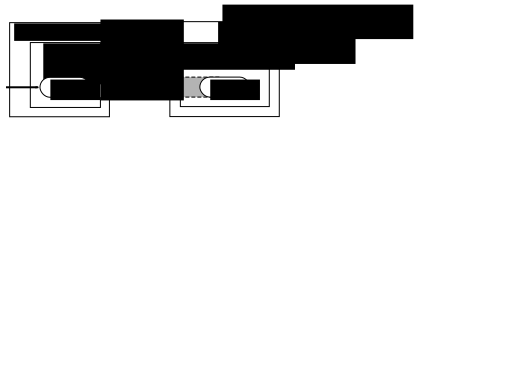
\includegraphics{./img/alsa-hw.svg.eps}
	\caption{{ALSA hw PCMプラグイン}}
	\label{fig:alsa-hw-plugin}
\end{figure}

ALSAアプリケーションがPCMインターフェイスAPIのopenを呼ぶと、この関数はランタイム設定ファイルを読んでパースする。ALSAのデフォルトでは、/usr/share/alsa/alsa.conf が最初にロードされる。このファイルは/usr/share/alsa/alsa.conf.d/*、/etc/asound.conf、~/.asoundrcを順にロードする。結果、PCMランタイムにおいていくつかのPCMノードが利用可能となる。例えば、hw、plughw (hwをスレーブとするplugプラグイン)、dmix、dsnoop、defaultだ。図\ref{pcm-nodes-playback}を参照のこと。


\begin{figure}[htbp]
\small
\begin{verbatim}
$ aplay -L
default:CARD=PCH
    HDA Intel PCH, CX20590 Analog
    Default Audio Device
...
dmix:CARD=Intel,DEV=0
    HDA Intel, ALC889 Analog
    Direct sample mixing device
dsnoop:CARD=Intel,DEV=0
    HDA Intel, ALC889 Analog
    Direct sample snooping device
hw:CARD=Intel,DEV=0
    HDA Intel, ALC889 Analog
    Direct hardware device without any conversions
plughw:CARD=Intel,DEV=0
    HDA Intel, ALC889 Analog
    Hardware device with all software conversions
\end{verbatim}
\caption{再生アプリケーションのALSA PCMノード}
\label{pcm-nodes-playback}
\end{figure}

\subsection{ALSA PCMプラグイン}
ALSAライブラリーはいくつかの目的のためのPCMプラグインを持つ\footnote{src/pcm/ in alsa-lib}。dmix/dsnoopプラグインはALSAプラグインのIPC仕様に関して、よい実例となる。dmixプラグインはいくつかのアプリケーションからのPCMフレームをマルチプレクスし、そのPCMフレームをデバイスに送信する。dsnoopプラグインはデバイスから受信したPCMフレームを複数のアプリケーションに配送する。dmix/dsnoopプラグインはSystem V共有メモリーをIPCに用い、System Vセマフォを相互排他に用いる。ALSA PCM directレイヤーはこれらプラグインのヘルパ関数を含む。


\begin{figure}[htbp]
	\centering
	\includegraphics[scale=0.75]{./img/alsa-direct.svg.eps}
	\caption{ALSA dmix PCMプラグイン}
	\label{alsa_direct}
\end{figure}


アプリケーションがsnd\_pcm\_open()を呼んでdmix/dsnoop PCMノードを開くと、dmix/dsnoopプラグインはSystem V共有メモリーとSystem Vセマフォを確保あるいは接続する。共有メモリーは各アプリケーションの仮想メモリー空間にアタッチされる。この共有メモリーはスレーブのPCMサブストリームのパラメータとステータスを共有するために用いられる。dmix/dsnoopのスレーブはhwプラグインに固定されている。加えて、dmixプラグインはマルチプレクス処理用バッファのために共有メモリーをもうひとつ確保する。

snd\_pcm\_writei()/snd\_pcm\_mmap\_commit()が呼ばれると、dmixプラグインはアプリケーションバッファーと共有メモリにあるPCMフレームをマルチプレクスし、スレーブバッファーに書き出す。このPCMフレームは共有メモリーに保存され、次のマルチプレクスの際に他のアプリケーションによって使われる。この共有メモリーはいわばキャッシュのようなものだ。これにより各プロセスは自分たちのタイミングでPCMフレームをマルチプレ薬師、フレームをスレーブのバッファーに書き込むことになる。スレーブのバッファーはhw PCMプラグインに寄って加えられたものだ。バッファーはプロセスの仮想アドレス空間にmmapされるため、どのプロセスも同じバッファーにアクセスすることになる (\pageref{fig:alsa-hw-plugin}ページの\ref{fig:alsa-hw-plugin}章)。dmixプラグインはPCMフレームを書き出す一方で、バッファーポインターを通常の方法で動かさない。これにより、複数のプロセスが同じ位置にPCMフレームを書き出すことができる。

dsnoop PCMプラグインはPCMフレームをマルチプレクスする必要がないため、dmix PCMプラグインよりも単純だ。それぞれのアプリケーションは共有メモリーからPCMフレームを読み出す。

私の目的にALSA PCMプラグインを使うには2つの問題がある。ALSA PCMプラグインの基本コンセプトは、hw PCMノードに機能を付与することだ。従って、ALSA PCMプラグインのフレームワークは、スレーブを伴わないマスターを許可しない。hw PCMノードはカーネルランドドライバーと通信するためのものであり、この章の私の目的に反している。加えて、ひとつのプロセスが必ずパケットを扱わなければいけないという問題がある。もしあるALSAアプリケーションがこの役割りを担った場合、他のアプリケーションがFireWireデバイスのためにPCMノードを使っている間、そのアプリケーションは終了することができない。従って、ALSAアプリケーションのためにパケットを扱うデーモンプロセスが必要となる。


\subsection{ALSA External PCMプラグイン}
ALSAはランタイムにPCMノードを拡張する方法をもうひとつ持っている。External PCMプラグインだ\cite{alsa-lib}。2つの使い方があり、ひとつはフィルター型、もうひとつはI/O型だ。

フィルター型プラグインはマスター/スレーブを伴うPCMプラグインに似ている。一方、I/O型はスレーブを伴わない。従ってI/O型は、デーモンプロセスとのコミュニケーションに適している。I/O型プラグインのよい実例は、PulseAudioのためのpulse PCM Externalプラグイン\footnote{pulse/ in alsa-plugins}だ。

PulseAudio\footnote{http://www.pulseaudio.org}はサウンドサーバーデーモンのプロジェクトだ。最近のデスクトップ環境では、PulseAudioがALSAランタイム設定\footnote{/usr/share/alsa/pulse-alsa.conf}を追加し、default PCMノードがpulse PCMノードとなるように上書きする。結果、デスクトップ環境のアプリケーションのほとんどは、pulse External PCMプラグインを経由して、PulseAudioとIPCする。そしてPulseAUdioがALSAアプリケーションのために、PCM標本をマルチプレクス/デマルチプレクスする。最後に、PulseAudioはそれぞれのデバイスに対し、PCM標本の転送を行う。

\begin{figure}[H]
	\centering
	\includegraphics[scale=0.5]{./img/alsa-pulse.dot.eps}
	\caption{ALSA pulse PCMプラグインとPulseAudio}
	\label{alsa-pulse}
\end{figure}

PulseAudioはRTP関連プロトコルのようなネットワークプロトコルを実装しており、またRygel\footnote{RygelはUPnP Device ArchitectureおよびMedia Renderer/ServerのためのDevice Control Protocolアプリケーション。}などの通信バックエンドを利用する。更に、PulseAudio自体が他のホスト上のPulseAudioと通信を行う独自のネットワークプロトコルを実装している。これは、PulseAudioがさまざまなデバイスを扱うフレームワークを持っていることを意味する。

他の実例がある。FreeBoBのためのfreebob External PCMプラグインだ。このプラグインのソースは、FFADOのsubversion repositoryのtrunkのalsa-pluginにある\footnote{http://subversion.ffado.org/browser/trunk}。

\begin{figure}[H]
	\centering
	\includegraphics[scale=0.5]{./img/alsa-freebob.dot.eps}
	\caption{{ALSA FreeBoB PCMプラグインとLinux firewireサブシステム}}
	\label{alsa_freebob}
\end{figure}

このプラグインは開始時にスレッドを設ける。このスレッドはlibfreebobのwait関数をpollし、起床する際にPCM標本とMIDIメッセージを転送する。このプラグインは再生と録音が可能ではあるもののまた、一度に1つのアプリケーションしかストレームを転送できないという制限がある。このアプリケーションはALSAシーケンサーインターフェイスを使い、他のALSAアプリケーションとMIDIメッセージの収集/配信を行う。このプラグインは途中で開発が終了したと思われるが、FFADOを利用するALSAアプリケーションを考える上で有用だ。

FreeBoB PCMプラグインはパケット処理を行うデーモンプロセスの必要性を強調する。何故なら、プラグインはPCMフレームの再生と録音を同時に扱えないからだ。最近のデスクトップ環境では、このようなデーモンとしてPulseAudioが候補に挙げられる。もしPulseAudioがfirewireスタックを持ったなら、ALSAアプリケーションはdefault PCMノードを経由してfirewireデバイスとデータの転送を行える。MIDI機能についてはFreeBoBプラグインがするように、PulseAudioもまたALSAのシーケンサーインターフェイスを使うべきだろう。

ところがすでに、似たようなPCM External I/Oプラグインが存在する。jackdのためのjack PCMプラグインだ。このプラグインはjack PCMノードをALSAランタイムに追加し、ALSAアプリケーションがjackdのクライアントとなるようにする。jackdはfirewireデバイスをFFADOバックエンドで利用可能だ。この方法はALSAランタイム設定をユーザーに求めるが、それ以上は求めない。

\begin{figure}[H]
	\centering
	\includegraphics[scale=0.5]{./img/alsa-jack.dot.eps}
	\caption{{ALSA JACK PCMプラグインとJACKサーバーデーモン}}
	\label{alsa_jack}
\end{figure}

しかしこの方法にも欠点がある。jackプラグインの設定を追加すると、jackdのプロセスがなくても、jack PCMノードが常にALSA PCMランタイム空間に出現する。これはユーザーにってのALSAアプリケーションの見通しを損なうことになる。


\subsection{CUSE - Character device in user-space}
Linuxのファイルシステムサブシステムは、FUSE拡張としてCUSEを持つ。CUSEはキャラクターデバイスドライバーをユーザーランドに実装することを可能にする。

\begin{figure}[H]
	\centering
	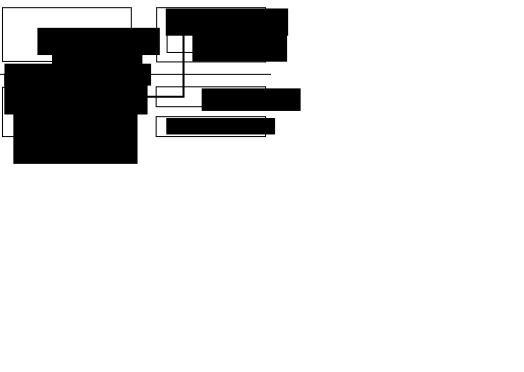
\includegraphics[scale=0.75]{./img/fuse.svg.eps}
	\caption{{FUSE/CUSEとユーザーランドドライバー}}
	\label{fuse}
\end{figure}

Open Sound System Proxy Daemon (osspd)はCUSEアプリケーションのよい実例である\footnote{http://sourceforge.net/projects/osspd/}。Open Sound SystemアプリケーションがOpen Sound Systemキャラクターデバイス (/dev/dsp, /dev/mixer, /dev/adsp)にアクセスすると、CUSEの助けを得たosspdがこれらのファイル操作をユーザースペースで扱い、PulseAudioあるいはALSAとIPCを行う。

\begin{figure}[H]
	\centering
	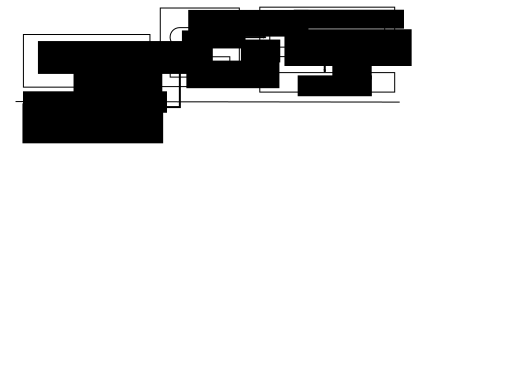
\includegraphics[scale=0.75]{./img/ossp-pulse.svg.eps}
	\caption{{Open Sound System Proxy Daemon}}
	\label{osspd_pulse}
\end{figure}

このデーモンはFUSEライブラリーAPIを用いて、Open Sound Systemキャラクターデバイスを登録する。udevデーモンはosspdが追加したルールに従い、これらのキャラクターデバイスをシステムに追加する。osspdはデーモンとスレーブの間のIPCを行うために一組のソケットを開き、スレーブのために新しいプロセスを開始する。このスレーブはデーモンからのIPCを待ち、PulseAudioあるいはALSAとIPCを行う。

私の目的にとって、この方法は素晴らしい。何故なら、ALSAのユーザーランド実装あるいはALSAのランタイムをいじる必要がないからだ。しかし、ALSAの全ファイル操作を扱うために、ALSA Coreと同等のコードがデーモンに実装されなければならない。これにはたくさんの労力が必要だ。この理由により、カーネルランドの軽量なALSAドライバーとALSA PCMコンポーネントのユーザーランド実装というのがよさそうである。


\begin{figure}[H]
	\centering
	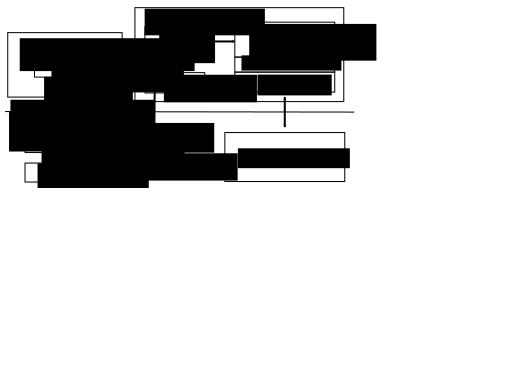
\includegraphics[scale=0.75]{./img/alsa-cuse-firewire.svg.eps}
	\caption{{CUSEを用いたALSA and Firewireのためのユーザーランドドライバー}}
	\label{alsa_cuse_firewire}
\end{figure}

デバイスが接続されると、このドライバーはPCMを除くALSAキャラクターデバイスを登録する。システムが新たなALSAのfirewireデバイスを検出すると、システムはデーモンを開始する。このデーモンはFUSEライブラリをコールし、ALSAのPCMキャラクターデバイスを適切なメジャー/マイナー番号と共に登録する。こうして、新しいPCMデバイスがALSAアプリケーションから利用可能となる。この案はデーモンのコードを減らすことができるが、ALSA PCMコンポーネントをデーモンに実装する作業が必要となる。

この章では、ALSAアプリケーションとfirewireドライバーのためのより良い方法を探すために、ユーザーランドのソフトウェア実装を調べた。結果、ドライバーをPulseAudioに実装することが最適な方法であるとの結論に達した。そしてそれは、ALSAのユーザーランド外の作業となる。次の章では、別な方法を探るために、ALSAのカーネルランド実装を調べる。

\section{カーネルランドドライバーの調査}

この章では、カーネルランドのALSA実装について調べる。

一般的に、システムコールを実行したプロセスはカーネルモードに遷移し、ハードウェア資源にアクセスする特権を得る。ハードウェアからのデータが到着していなければ、プロセスはプロセススケジューラーに依頼し、コンテキストスイッチを実行させる。そして他のプロセスがCPUを獲得して走り始める。休眠する前プロセスは、起床するイベントを登録する。コンテキストスイッチがリクエストされる度に、プロセススケジューラーはそのイベントをチェックし、どのプロセスを起床させるか決定する。これはプロセス数じけジューリングの一部であり、タイムシェアリングシステム (TSS) に貢献する

ALSAのアプリケーションがシステムコールを実行すると、カーネルモード中のプロセスはALSA Coreのコードに到達する。ALSA CoreはPCMなどのインターフェイスに対応するモジュールを含んでいる。これらのモジュール内のコードがイベントをチェックし、もしイベントが発生していたらプロセスを継続する、もしイベントが発生していなかったらプロセスを休眠させる。サウンドデバイスがハードウェア割り込みを発生させると、それぞれのALSAドライバーはこれをハンドルし、イベントを発生する。これがカーネルランドのALSA実装の簡単な説明である。

\subsection{ALSA Coreとドライバー}

ALSA Coreはサウンドサブシステムにおいて重要な役割りを果たすモジュールで構成されている。ALSA Coreのソースコードはsound/core/以下に配置されている。ALSA Coreはサウンドデバイスを「カード」として管理し、そのカードに含まれる「コンポーネント」に対応するキャラクターデバイスを管理する\cite{alsa-driver}。コンポーネントとは、PCMやMIDIなど、サウンドデバイス上の各機能を表すもので、モジュールはそれぞれのコンポーネントのヘルパー関数を含む。

サウンドデバイスが検出されると、対応するドライバーがカードのインスタンスをALSA Coreに登録し、コンポーネントのインスタンスをカードに登録する。そしてALSA CoreはLinux Driver Coreに倒し、キャラクターデバイスをシステムに追加するよう依頼する。この依頼が認められて処理されると、Linux Driver Coreはキャラクターデバイスを登録し、対応するkobjectを追加してkeventを通知する。通常のデスクトップ環境では、udevdがkeventを受信し、個別のルールに従ってシステムにスペシャルファイルを追加する。こうして、ALSAアプリケーションはスペシャルファイルを通じてドライバーのコンポーネントと通信できるようになる。

ALSA Coreの主要なモジュールは以下だ:

\begin{description}
\small
\item[snd] \mbox{} \\
カードとデバイスを管理。controlインターフェイスのメソッドと、controlコンポーネントのヘルパー関数、procfsのヘルパ関数を含む。
\item[snd\_pcm] \mbox{} \\
PCMインターフェイスのメソッドと、PCMコンポーネントのヘルパー関数を含む。
\item[snd\_rawmidi] \mbox{} \\
MIDIインターフェイスのメソッドと、MIDIコンポーネントのヘルパー関数を含む。
\item[snd\_hwdep] \mbox{} \\
hardware dependentインターフェイスのメソッドと、hardware dependentコンポーネントのヘルパー関数を含む。
\item[snd\_timer] \mbox{} \\
timerインターフェイスのメソッドと、timerコンポーネントのヘルパー関数を含む。
\end{description}

これらのコンポーネントは、ioctlやmmapといったLinuxのファイルシステム共通のファイル操作のメソッドを含み、ドライバーに向けてALSA固有の操作を定義する。それぞれのドライバーはコンポーネントを追加する際、コールバック関数をメソッドとして追加する。このようにして、それぞれのドライバーはALSAアプリケーションからの要求を処理できるようになる。

実際のデバイスと通信するために、ドライバーはそれぞれのLinuxサブシステムを使う。デバイスはPCI-Expressバスやplatformバスの上にあるからだ。ドライバーはバスドライバーに対して登録を行い、バスドライバーからのコールバックを処理する。加えてデータ転送はたいていDMAに基づいて行われ、関連するイベントはハードウェア割り込みによって通知される。それぞれのドライバーはDMAとハードウェア割り込みを処理するために、Linuxのサブシステムを使う。

次の説では、PCMインターフェイス/コンポーネントとアプリケーション/ドライバーに付いて述べる。


\subsection{ALSA PCMインターフェイスとPCMコンポーネント}
\label{sec:alsa-pcm}

ALSA PCMインターフェイスとPCMコンポーネントは、アプリケーションとデバイスの間でPCMフレームの転送を行うためのものだ。

PCMコンポーネントのインスタンスは、PCMストリームのための2つのメンバーを持つ。ひとつは入力ストリームのための、もうひとつは出力ストリームのためのものだ。デバイスの仕様に応じて、ドライバーは、ひとつのPCMストリームに複数のPCMサブストリームを追加する。サブストリームのために、ALSA CoreはPCMキャラクターデバイスを追加する。アプリケーションがPCMインターフェイスを使ってPCMキャラクターデバイスを開くと、対応するPCMサブストリームが開かれ、PCMランタイムがそのPCMサブすストリームにアタッチされる。

PCMランタイムはいくつかの状態を持つ。open、setup、prepared、running、xrun、draining、paused、suspend、disconnectedだ\cite{alsa-lib}。アプリケーションはPCMインターフェイスを使って状態を変更し、その時ドライバーの対応するメソッドがPCMコンポーネントのインスタンスによってコールされる。ランタイムはハードウェアの詳細やハードウェア/ソフトウェアパラメータなどの情報を含む。ランタイムが作成されると、ドライバーはハードウェア詳細をランタイムに追加する。次に、アプリケーションがPCMインターフェイスを使い、ハードウェア/ソフトウェアパラメータをセットする。

パラメータが決定すると、PCMリングバッファが確保される。大抵の場合、ドライバーはPCMコンポーネントのためのmmapファイル操作をサポートする。アプリケーションあるいはマスタープラグインがmmapアクセスフラグをハードウェアパラメータ\footnote{SND\_PCM\_ACCESS\_MMAP\_INTERLEAVED, SND\_PCM\_ACCESS\_MMAP\_NONINTERLEAVED and SND\_PCM\_ACCESS\_MMAP\_COMPLEX}に追加した場合、PCMインターフェイスはこのバッファーをプロセスの仮想アドレス空間にマップする。

リングバッファーの状態は他のバッファー上にある。statusバッファーとcontrolバッファーだ。これらのバッファーはアプリケーションあるいはmasterプラグインがhwプラグインを開く際、PCMコンポーネントによってカーネルスペースに設けられる。そして、大抵の場合、これらバッファーのhw\_ptrとappl\_ptrがプロセスの仮想アドレス空間にマップされる\footnote{mmap(2)の実行に失敗した場合、代わりの方法が適用される。hwプラグインはsync\_ptr構造のバッファを一つ確保する。PCMフレームを読み書きした際、このポインターを更新するioctl(2)が実行される。この方法はオーバーヘッドを含む。}


\begin{figure}
\small
\begin{verbatim}
struct snd_pcm_mmap_status {
        snd_pcm_state_t state;
        int pad1;
        snd_pcm_uframes_t hw_ptr;
        struct timespec tstamp;
        snd_pcm_state_t suspended_state;
        struct timespec audio_tstamp;
};
\end{verbatim}
\begin{verbatim}
struct snd_pcm_mmap_control {
        snd_pcm_uframes_t appl_ptr;
        snd_pcm_uframes_t avail_min;
};
\end{verbatim}
\caption{{リングバッファーステータスおよびコントロールためのデータ構造}}
\label{pcm-mmap-status-control}
\end{figure}

appl\_ptrはアプリケーションによってのみ更新される。2つの場合があり、ひとつはPCMフレームがnon-mmap関数で書き込まれたあるいは読み出された場合だ\footnote{snd\_pcm\_writei() / snd\_pcm\_writen() / snd\_pcm\_readi() / snd\_pcm\_readn()。ただしプラグインチェーンを考慮せよ。}。この場合、要求されたフレーム数だけ、カーネルスペースでPCMコンポーネントがappl\_ptrを動かす。もうひとつはフレームがmmap関数によりコミットされた場合だ\footnote{snd\_pcm\_mmap\_commit()。ただしプラグインチェーンを考慮せよ。}。この場合は、要求されたフレーム数だけ、ユーザースペースでhwプラグインがappl\_ptrを動かす。

一方でhw\_ptrは、デバイスからのハードウェア割り込みをハンドルしたドライバーによってのみ変更される。hw\_ptrを含むメモリーページはユーザースペースに読み込み限定でマップされ、アプリケーションは変更することができない。hw\_ptrはperiodのフレーム数だけ更新される。periodはリングバッファを分割した一部だ。デバイスがperiodのフレーム数だけPCMフレームを転送し終えた事を確認すると、snd\_pcm\_period\_elapsed()を呼ぶ。そしてhw\_ptrが次のperiodの最初に移動する。


\begin{figure}[H]
	\centering
	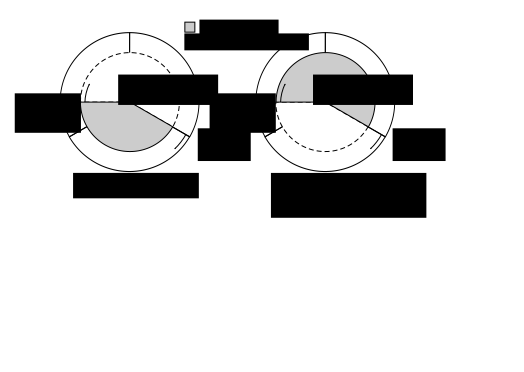
\includegraphics{./img/alsa-pcm-buffer.svg.eps}
	\caption{{PCMリングバッファー}}
	\label{alsa-pcm-buffer}
\end{figure}

2つのポインター、hw\_ptrとappl\_ptrはアプリケーションのavailスペースを確認するために用いられる。availスペースは現在アプリケーションが利用可能なフレーム数のことだ。再生アプリケーションにとっては、availスペースはリングバッファー上のPCMフレームが書き込まれていないスペースと等しい。録音アプリケーションにとっては、availスペースはPCMフレームが書き込まれているスペースと等しい。hwプラグインがnon-blocking操作でフレームの書き込みや読み出しを行った時、availスペースが要求フレーム数に満たなかった場合は、関数は即座に返る。blocking操作の場合は、要求フレーム数がすべて転送されるか、タイムアウトとなるまで、アプリケーションは待たされる。デフォルトでは、このタイムアウトは10秒となっている。タイムアウトはhw\_ptrが10秒間更新されなかったことを意味するため、割り込みハンドラーに関する何らかの問題が発生しているだろう。

だが、この挙動はNO\_PERIOD\_WAKEUPフラグをハードウェアパラメーターに設定することで変更できる\footnote{SNDRV\_PCM\_HW\_PARAMS\_NO\_PERIOD\_WAKEUP}。もしドライバーがこの機能をサポートしていたら、タイムアウトはLinuxのプロセススケジューラーがサポートする最大値\footnote{MAX\_SCHEDULE\_TIMEOUT in include/linux/sched.h}となる。このモードでは、ハードウェア割り込みは定期的に発生しなければならないし、ドライバーは必ずそれをハンドルしなければならない。

アプリケーションがhwプラグインがsnd\_pcm\_poll\_descriptors()によって返したディスクリプターに対してpoll(2)を実行すると、デフォルトでは、タイムアウト、availスペースが余裕を持つ、シグナルを受信のいずれかのイベントが起こるまでプロセスはブロックする。この挙動に対し、PCMコンポーネントは2つの挙動を持つ。一つはこれまで述べたような割り込みベースなモード、もうひとつは割り込みベースとタイマーベースの組み合わせモードだ。後者においては、snd\_pcm\_poll\_descriptors()はPCMキャラクターデバイスとTimerキャラクターデバイスの2つのディスクリプターを返す。どちらもピリオド単位で起床するが、タイマー源が異なる。モードの変更はsnd\_pcm\_sw\_params\_set\_period\_event()を実行することによりperiod\_eventソフトウェパラメータを設定して行う。PulseAudioは先述したNO\_PERIOD\_WAKEUPハードウェアパラメータとperiod\_eventソフトウェアパラメータを用い、glitch free操作を実現している\footnote{Features/GlitchFreeAudio http://fedoraproject.org/wiki/Features/GlitchFreeAudio}。

リングバッファ上のavailに対する残りはhw\_availだ。これはデバイスにとって利用可能なスペースのことだが、アプリケーションにとっては巻き戻し(rewind)のためのスペースとなる。アプリケーションはhw\_availのフレーム数を上限に、appl\_ptrを戻すことができる。この時、開発者はhw\_ptrはいつでもドライバーによって変更される可能性があることを年頭に置かなければならない。


これら2つのポインタの値は、バッファーのフレーム数でラウンドアップするわけではない。UINT\_MAX内のboundaryまで増加し、そこでラウンドアップする。boundaryの算出式は以下だ:

\begin{equation}
boundary = UINT\_MAX - UINT\_MAX / frames\_per\_buffer 
\end{equation}

\begin{figure}[H]
	\centering
	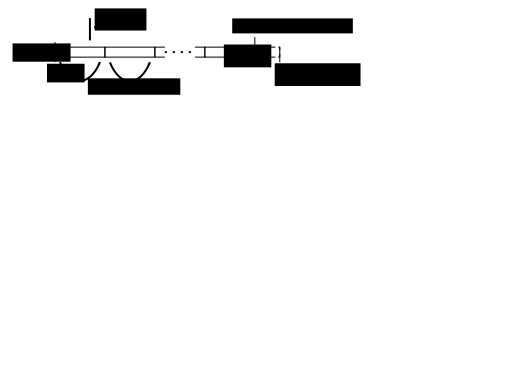
\includegraphics{./img/alsa-buffer-boundary.svg.eps}
	\caption{{PCM buffer boundary}}
	\label{alsa--buffer-boundary}
\end{figure}


\subsection{Linux firewireサブシステム}

ALSAのfirewireスタックはLinux firewireサブシステムを使い、FireWireデバイスと通信する。ALSAのfirewireスタックを調査する前に、Linux firewireサブシステムについて述べる。

Linux firewireサブシステム - Juju\footnote{由来は知らない}と呼ばれる - は、IEEE 1394ちOHCI 1394のアプリケーションであり、以下の機能をサポートする:

\begin{itemize}
\small
\item IEEE 1394シリアルバス管理
\item IEEE 1394トランザクション層
\item OHCI 1394準拠コントローラーデバイスドライバー
\item unitに対応するfwキャラクターデバイスドライバー
\end{itemize}

このサブシステムはdrivers/firewire/にあり、いくつかのファイルから成る。また、特定の1394コントローラーがサポートするsnoopモードに対するドライバーや、RFC 2734\footnote{https://tools.ietf.org/html/rfc2734 IPv4 over IEEE 1394}、RFC 2855\footnote{https://tools.ietf.org/html/rfc2855 DHCP for IEEE 1394}、RFC 3146\footnote{https://tools.ietf.org/html/rfc3146 Transmission of IPv6 Packets over IEEE 1394 Networks}そしてSBP-2などのプロトコルドライバーも含む。ここではコア機能とOHCI 1394関係コードについてのみ述べる。

\begin{description}
\small
\item[drivers/firewire/core-cdev.c] \mbox{} \\
fwキャラクターデバイスのファイル操作のためのメソッドを含む。
\item[drivers/firewire/core-device.c] \mbox{} \\
unit管理のためのヘルパーファンクションを含む。
\item[drivers/firewire/core-topoligy.c] \mbox{} \\
バスのイベントに応じてバストポロジーを管理する。
\item[drivers/firewire/core-iso.c] \mbox{} \\
アイソクロナスコンテキストを扱うヘルパー関数を含む。
\item[drivers/firewire/core-transaction.c] \mbox{} \\
アシンクロナスコンテキストを扱うヘルパー関数を含む。
\item[drivers/firewire/core-card.c] \mbox{} \\
ホストコントローラーデバイスのための抽象レイヤー。
\item[drivers/firewire/ohci.c] \mbox{} \\
OHCI 1394準拠ホストコントローラードライバー。
\end{description}

\begin{figure}[htbp]
	\centering
	\includegraphics[scale=0.5]{./img/fw-stack-high.dot.eps}
	\caption{{Linux firewireサブシステム(上部)}}
	\label{fw-stack-high}
\end{figure}

このサブシステムはIEEE 1394のcycle masterとバス管理を行う。また、アプリケーションのためにfwキャラクターデバイスを設ける。fwキャラクターデバイスはIEEE 1394バス上のそれぞれのユニットに対応する。ユーザーランドのアプリケーションはこれらfwキャラクターデバイスに対してファイル操作 - 主にioctl(2) - を実行し、ユニットと通信を行うことができる。ALSAがそうであるようにこのサブシステムも、ファイル操作の抽象レイヤーとして入出力ライブラリー (libraw1394) を提供する。加えて、このシステムはカーネルランドにもAPIを提供する。

アシンクロナスとアイソクロナス通信機能はOHCI 1394に基づいており、コンテキストとして表現される (\pageref{ohci-1394}ページの\ref{ohci-1394}章)。

Linux firewireスタックはコントローラーデバイスの抽象レイヤーも持つ。現在は2つのドライバーがこの抽象レイヤーの下にある。dummyドライバーは主に実際のカードを終了する際に用いられているため、OHCI 1394ドライバーが実際のデバイスとの通信に用いられる。このドライバーはディスクリプターに従ってDMAによってコントローラーとパケットの送受信を行い、コントローラーが発生するハードウェア割り込みをハンドルする。ドライバーはレジスターによりコントローラーを制御する。

\begin{figure}[htbp]
	\centering
	\includegraphics[scale=0.5]{./img/fw-stack-low.dot.eps}
	\caption{{Linux firewireサブシステム (下部) とホストコントローラー}}
	\label{fw-stack-low}
\end{figure}

\subsection{ALSA firewireスタック}

ALSAのfirewireスタックはLinux firewireサブシステムを使ってFireWireデバイスと通信するドライバーのために設計された。このスタックはsound/firewire/以下にある。このスタックはIEC 61883-1/6のヘルパー関数を含む。

\begin{description}
\small
\item[sound/firewire/iso-resources.c] \mbox{} \\
   アイソクロナス資源を管理するヘルパー関数を含む。
\item[sound/firewire/cmp.c] \mbox{} \\
   IEC 61883-1のConnection Management Procedure (CMP)のためのヘルパー関数を含む。
\item[sound/firewire/lib.c] \mbox{} \\
   アイソクロナストランザクションのためのヘルパー関数を含む。
\item[sound/firewire/fcp.c] \mbox{} \\
   IEC 61883-1のFunction Control Protocolのためのヘルパー関数を含む。
\item[sound/firewire/packets-buffer.c] \mbox{} \\
   連続したパケットのためのバッファーを管理するヘルパー関数を含む。
\item[sound/firewire/amdtp.c] \mbox{} \\
   IEC 61883-6のAMDTPパケットストリーミングのためのヘルパー関数を含む。
\end{description}

これらの全てはsnd-firewire-libモジュールをビルドするために使われる。firewireサウンドドライバーはサウンドデバイスと通信するためにこれらのヘルパー関数を使う一方、ALSAアプリケーションと通信するためにALSA Coreも用いる。

\begin{figure}[htbp]
	\centering
	\includegraphics[scale=0.5]{./img/alsa-stack.dot.eps}
	\caption{{ALSA Coreとfirewireスタック}}
	\label{alsa_stack}
\end{figure}

\subsubsection{Isochronous資源機能}

このモジュールはチャンネルとバンド幅というアイソクロナス資源のためのデータ構造を提供する。ドライバーはfw\_iso\_resources\_init()を使ってこのデータ構造のインスタンスを初期化する。そして、fw\_iso\_resources\_allocate()とfw\_iso\_resources\_free()を使ってアイソクロナス資源のアロケートと解放を行う。バスリセット発生時は、fw\_iso\_resources\_update()を呼ばなければならない。インスタンスを開放するには、fw\_iso\_resources\_destroy()を用いる。

\subsubsection{CMP機能}

このモジュールはCMP操作のためのデータ構造を提供する。この機能はアイソクロナス資源機能を内部で用いる。ドライバーはcmp\_connection\_init()を用い、このデータ構造のインスタンスを初期化する。そして、パケットのペイロードの最大バイト数をcmp\_connection\_establish()に与え、バンド幅およびチャンネルの確保と接続を行う。コネクションの切断には、cmp\_connection\_break()を用いる。インスタンスの解放には、コネクションを切断した後でcmp\_connection\_destroy()を用いる。バスリセットが発生した場合は、コネクションを更新するためにcmp\_connection\_update()を用いる。

2013年現在、この機能は入力コネクションのためのiMPR/iPCRに対する操作をサポートする。

\subsubsection{FCPとトランザクション機能}

FCP機能はひとつの関数 - fcp\_avc\_transaction() - をFCPとAV/Cコマンドのために提供する。ドライバーはFCPリクエストを送信し、FCPレスポンスを125ミリ秒待つ。バスリセット発生時、すべてのFCPリクエストはリトライされる。このために、fcp\_bus\_reset()が用いられる。

FCP機能は内部ではsnd\_fw\_transaction()を用いる。これはfw\_run\_transaction()のラッパー関数であり、リトライとバスの世代制限をサポートする。


\subsubsection{連続したパケットのためのバッファー機能}

このモジュールは連続したパケットのバッファーのためのデータ構造を提供する。ドライバーは、パケット数と1パケットあたりのバイト数をiso\_packets\_buffer\_init()に与え、このデータ構造のインスタンスを初期化する。初期化の後、インスタンスはパケットをキューイングするためのページを持つ。このインスタンスを開放するには、iso\_packets\_buffer\_destroy()を用いる。

\subsubsection{AMDTP機能}
\label{sec:packetization-out}

このモジュールはAMDTP出力ストリームのためのデータ構造および操作を提供する。この機能は連続したパケットバッファー機能を内部で用いる。ドライバーはamdtp\_out\_stream\_init()を用い、このデータ構造のインスタンスを初期化する。初期化の後、サンプリング周波数やMBLAデータチャンネル数、MIDI Conformantデータチャンネル数などのストリーミングパラメータをセットするために、amstp\_out\_stream\_set\_parameters()を用いる。パラメータをセットした後、amdtp\_out\_stream\_get\_max\_payload()は現在のパケットのペイロードの最大バイト数を返す。

ドライバーはamdtp\_out\_stream\_start()を用い、ストリームを開始する。ストリームを止めるにはamdtp\_out\_stream\_stop()を用いる。インスタンスを開放するにはamdtp\_out\_destroy\_stream()を用いる。バスリセットが発生した場合は、amdtp\_out\_stream\_update()を用いてノードIDを更新する。

PCMコンポーネントのために、snd-firewire-libはヘルパー関数提供する。ストリームを開始する前に、amdtp\_out\_stream\_set\_pcm\_format()を用いてPCMのフォーマットをセットする。インスタンスのPCM関係メンバーを初期化するために、amdtp\_out\_stream\_pcm\_prepare()を用いる。PCMフレーム転送の開始/終了には、amdtp\_out\_stream\_pcm\_trigger()を用いる。PCMリングバッファ上のフレーム数を取得するには、amdtp\_out\_stream\_pcm\_pointer()を用いる。PCMサブストリームを殺すには、amdtp\_out\_stream\_pcm\_abort()を用いる。PCMサブストリームがAMDTPストリーム上に流れているかどうかを確認するには、amdtp\_out\_stream\_pcm\_running()を用いる。

AMDTP出力パケットの生成の詳細を、図\ref{fig:packetization-out}に示す。まず、amdtp\_out\_stream\_start()がskipフラグと共に、一連のパケットをキューイングする。すると、firewire-ohciがこれらのパケットをディスクリプターリストに登録する。最後のパケットにはinterruptフラグを付与し、このinterruptパケットがキューされたとき、firewire-ohciがこのパケットに対応するディスクリプターに特別なフラグを付与するようにする。キューイングの後、amdtp\_out\_stream\_start()関数はコールバック関数と伴にアイソクロナスコンテキストを開始する。そして、firewire-ohciはOHCI 1394コントローラーへのDMAによるディスクリプターの転送を開始する。OHCI 1394コントローラーはこのディスクリプターに対応するパケットを転送する。OHCI 1394コントローラーはinterruptパケットを転送し終えると、ハードウェア割り込みを発生する。firewire-ohciはこの割り込みをハンドルし、taskletをスケジュールする。このtaskletがソフトウェア割り込みコンテキストで実行されると、コールバック関数が実行される。snd-firewire-libは新たな一連のパケットをPCMフレームと共に生成し、それらをキューイングする。最後のパケットは再びinterruptフラグが付与される。OHCI 1394コントローラーがこのパケットの転送を終えると、ハードウェア割り込みを発生し、snd-firewire-libは新たな一連のパケットを生成してキューイングする。

\begin{figure}[H]
	\centering
	\includegraphics{./img/packetization-out.svg.eps}
	\caption{{出力ストリームパケットの生成}}
	\label{fig:packetization-out}
\end{figure}

2013年現在、AMDTP機能は1キューを48パケット\footnote{QUEUE\_LENGTH in sound/firewire/amdtp.c}で構成し、16パケット毎にinterruptフラグを立てる\footnote{INTERRUPT\_INTERVAL in sound/firewire/amdtp.c}。ハードウェア割り込みはnominal値で2ミリ秒ごとに発生し、アイソクロナスコンテキストが開始されてからPCMフレームを伴う最初のパケットが転送されるまで6ミリ秒かかる。実際のハードウェア割り込みインターバルはバンド幅使用率 (\pageref{fig:cycle-start}ページの図\ref{fig:cycle-start}) とtaskletスケジューリングに依存している。

snd-firewire-libがストリーミングの持続に失敗する場合がある。それはパケットのキューイングに失敗した場合だ。ストリームが止まっているかどうかを判定するために、amdtp\_out\_stream\_running()を用いる。amdtp\_out\_streaming\_error()はエラーの検出に用いる。一度ストリーミングがエラー状態となったら、amdtp\_out\_stream\_stop()で止めてからamdtp\_out\_stream\_start()で再開しなければならない。


2013年現在、この機能はドライバーがタイミングスレーブとして振る舞うことを許可していない。タイミングスレーブは入力パケットのSYTフィールドから出力パケットのSYTフィールドの値を生成しなければならない (\pageref{sec:duplex-streams}ページの\ref{sec:duplex-streams}章) が、この機能は入力ストリームをサポートしていないからだ。従ってこの機能は、SYTフィールドの値と1パケットのデータブロック数の生成器を持つ。これらの値は互いに関係するからだ。


\section{ALSAのfirewireスタックの改良}

2013年時点で、このスタックはAMDTP出力ストリーム - デバイスの視点に立てば受信ストリーム - のみを、blocking/non-blockingモードのどちらでもサポートする。詳細を見ると:

\begin{itemize}
\item iMPR/iPCRだけを扱うCMP機能
\item アイソクロナス出力コンテキストだけを扱うAMDTP機能
\item PCMフレームだけを転送するAMDTPパケット
\item 入力パケットのSYTフィールド値を出力パケットに利用できない。
\end{itemize}

より多くのデバイスをサポートするために、このスタックは以下の機能を必要とする:
\begin{itemize}
\item oMPR/oPCRを扱う機能
\item アイソクロナス入力コンテキストを扱う機能
\item MIDIのような、様々なデータをAMDTPパケットで扱う機能
\item タイムスタンプ同期を伴う全二重ストリーム
\end{itemize}

加えて、それぞれのドライバーは以下の機能を必要とする:
\begin{itemize}
\item デバイスのケーパビリティを取得しそれをパースし、PCMランタイムルールを作る機能
\item 全二重ストリームのサポート
\item 再生と録音、両方をサポートするPCMコンポーネント
\item 再生と録音、両方をサポートするMIDIコンポーネント
\item モデル固有の操作と癖を扱う機能
\end{itemize}

更に、それぞれのドライバーはユーザーランドドライバーを妨害してはならない。Diceドライバーは既に、hwdepインターフェイスを通じて以下の機能を提供している:
\begin{itemize}
\item ALSAカードに伴うfirewireノード情報を提供する機能
\item ストリーミングの開始、終了を通知する機能
\item ストリーミングのロックと解放
\end{itemize}

ドライバーをユーザーランドに実装するという発想と比較すると、カーネルランドに実装するという発想の方が、ALSA Coreを使うことができるため、ALSAアプリケーションとの通信において課題がより少ない。この発想はALSAアプリケーションによりよい見通しを与える。更に、すでにALSAのfirewireスタックがある。このスタックはいくつかの要求を満たさないものの、ユーザーランドにドライバーを実装するよりも少ない労力で改良できる。

私はこの発想に基づき、2013年にこの仕事を始めた。この仕事は2014年にALSAの上流にマージされた。1年半かかっている。2014年6月のLinux 3.16のマージウィンドウにおいて、ALSAのメンテナーはこの仕事をLinuxの上流にプッシュされた。この仕事のパッチセットはたくさんのパッチに沸かれている。最初の18パッチはsnd-firewire-libのAMDTP、CMP、FCPのためのものだ。次の14パッチはfireworksドライバーの、続く16パッチはBeBoBドライバーのためのものだ。残りのパッチはバグ修正だ。

\subsection{Enhancement for AMDTP}

The snd-firewire-lib newly supports these functionalities for AMDTP:

\begin{itemize}
	\item Handling incoming AMDTP stream
	\item PCM capturing support
	\item MIDI capturing/playbacking support
	\item AMDTP data channel mapping
	\item duplex streams with timestamp synchronization
\end{itemize}

This work renames prefix of 'amdtp\_out\_stream' to 'amdtp\_stream' for all of functions and members for AMDTP stream structure, to use the same structure and functions for both directions.

This work newly adds a support for AMDTP incoming stream, and adds an argument for amdtp\_stream\_init(), to indicate the direction of AMDTP stream. After initialized, the instance of stream can be operated by the same way for both direction.

Let's see the detail to handle AMDTP incoming stream in Figure \ref{fig:packetization-in}. The mechanism is almost the same as generating outgoing packets, while there are two big differences.

One is dequeueing packets instead of generating packets. When OHCI 1394 controller fills an 'interrupt' descriptor with an incoming packet, it generates a hardware interrupt. The firewire-ohci handles this hardware interrupt and schedules tasklet. When the tasklet is executed in software interrupt context, a callback function in snd-firewire-lib is executed. Then AMDTP functionality perform dequeueing and queueing packets.

In current implementation, the length of queue and the interval of interrupt is the same for incoming/outgoing AMDTP stream. As a result, it nominally takes 2 millisecond to handle a first incoming packet since the packet reached.

Another is a functionality to detect discontinuity of the sequence of incoming AMDTP packets. Each AMDTP packet has DBC field for this purpose. In a case of the detection, the stream is stopped and corresponding PCM substream is aborted. In this case, the stream should be stopped and started again.

\begin{figure}[H]
	\centering
	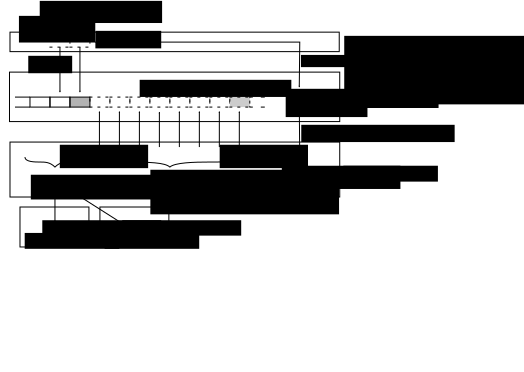
\includegraphics{./img/packetization-in.svg.eps}
	\caption{{Handling packets for incoming stream}}
	\label{fig:packetization-in}
\end{figure}

This work newly adds amdtp\_stream\_wait\_callback() to wait for a first packet until given timeout. This is for detection of the case that drivers set wrong parameters for packets, i.e. a wrong tag for IEEE 1394 isochronous packet. In this case, OHCI 1394 driver doesn't execute callback function in isochronous context. Then no packets are handled, and PCM component don't waken a process of PCM substream because 'avail' space has never been updated (section \ref{sec:alsa-pcm} to page \pageref{sec:alsa-pcm}). This function is expected to be used just after staring a stream, to prevent from this case. Drivers should handle error state when receive false.

This work adds some flags for AMDTP stream structure, to handle device's quirks of stream. Between initializing and starting a stream, these flags can be set to an instance of the stream. Fireworks and BeBoB drivers use these flag.

By default, any AMDTP streams are not associated. For duplex streams with timestamp synchronization (section \ref{sec:duplex-streams} to page \pageref{sec:duplex-streams}), amdtp\_stream\_set\_sync() is added to associate two streams as a timing master and a timing slave with given synchronization mode, and this function should be called before starting streams. Currently CIP\_SYNC\_TO\_DEVICE is effective for this parameter and for AMDTP stream in blocking mode. The case to use this option is that a timing master is incoming stream and a timing slave is outgoing stream. In this case, the value of SYT field in incoming packets are passed to outgoing packets. The packets in both direction are handled in interrupt context for an incoming isochronous context. Hence, a callback in isochronous context for outgoing stream is ignored. In the other cases, there's no requirement to pass the value of SYT field between two streams.

\begin{figure}[H]
	\centering
	
\includegraphics{./img/packetization-duplex.svg.eps}
	\caption{{Handling associated duplex streams}}
	\label{fig:packetization-duplex}
\end{figure}


In IEC 61883-6\cite{iec61883-6-1, iec61883-6-2} and MMA/AMEI RP-027\cite{amei-rp27}, one MIDI Conformant data channel supports 8 MIDI substreams. This work newly adds a support of this multiplexed MIDI substream in AMDTP stream. During streaming, each drivers can trigger MIDI messages with amdtp\_stream\_midi\_trigger(). Some models ignore MIDI messages in more than 8 data blocks in an packet. This may be due to a gap of data rate between MIDI bus and IEEE 1394 bus. To handle this quirk, struct amdtp\_stream.rx\_blocks\_for\_midi is used.

For PCM component, this work newly adds amdtp\_stream\_add\_hw\_constraints() to add PCM constraint according to parameters of AMDTP stream. This function should be called after all of needed flags are set to an instance of AMDTP stream structure.

This work allows drivers to call amdtp\_stream\_set\_pcm\_format() during a stream is running. This is for the case that PCM substream is going to join in AMDTP stream which MIDI substream already starts.

\subsection{Enhancement for CMP}

This work adds an argument to cmp\_connection\_init(), to indicate direction. After initializing, the instance of CMP is handled as what it was.

Each driver can read iPCR/oPCR by transaction in any time. To confirm no drivers handle the device, cmp\_connection\_check\_used() is used. This is a consideration about user-land driver. I also proposed the same idea for FFADO\footnote{[FFADO-devel] Adjustment between FFADO/ALSA for Firewire drivers  http://sourceforge.net/p/ffado/mailman/message/31856195/}.

I note that the value of payload field in oPCR is not used to keep bandwidth because some device chip reports a wrong value. Instead of this, snd-firewire-lib uses the value of data\_block\_quadlets member in struct amdtp\_stream.

\subsection{Enhancement for FCP}

This work enables firewire-lib to handle deferred transaction. According to AV/C General specification\cite{avc-general-4-2}, receivers of AV/C command should respond to transmitter within 100 millisecond, while the receivers send an intermediate response within 100 millisecond and send a final response later. This is deferred transaction. The interval between the intermediate and the final response is undefined. But to promise to return to caller, 125 millisecond interval is used.

Additionally, this work adds three AV/C commands, which seems to be used in some drivers. They are INPUT/OUTPUT SIGNAL FORMAT command and PLUG INFO command in AV/C General\cite{avc-general-4-2}.

\section{Driver implementation}

The enhancement of ALSA firewire stack allows to implement new drivers and to update existed drivers. In this section, I describe about specifications of these drivers.

\subsection{Common specifications}

The drivers for Fireworks/BeBoB/OXFW/Dice utilize ALSA firewire stack, therefore they have common specifications for each component.

\subsubsection{PCM component}

An instance of PCM component in each driver has SND\_PCM\_INFO\_BATCH flag because AMDTP functionality uses several packet buffers to transfer PCM frames (section \ref{sec:alsa-pcm} to page \pageref{sec:alsa-pcm}).

PCM component also has SND\_PCM\_INFO\_BLOCK\_TRANSFER flag because PCM frames are transferred at each interrupt by the number of data blocks in some packets \footnote{INTERRUPT\_INTERVAL in /sound/firewire/amdtp.c}.

PCM frames are copied to each data blocks in its order and the position of PCM frames in a data block is linear, thus SNDRV\_PCM\_INFO\_INTERLEAVED should be used.

If devices supports both streams, in most case, incoming/outgoing AMDTP streams should be the same sampling rate, thus SNDRV\_PCM\_INFO\_JOINT\_DUPLEX should be used. Each drivers should restrict sampling rate for both playback/capture as the same. If current source of clock is not internal or recovered clock (section \ref{sec:clock-recovery} to page \pageref{sec:clock-recovery}), the sampling rate should not be changed.

Currently, SNDRV\_PCM\_HW\_PARAMS\_NO\_PERIOD\_WAKEUP is not used because these drivers have a possibility to stop streaming suddenly due to failure of packet queueing or detection of packet discontinuity. In this case, process with the flag is kept blocking.

The number of channels in each PCM substream depends on the number of MBLA data channels in data block of AMDTP packet. The number is different depending on models even if the models use the same device chipset (Section \ref{sec:formation-data-block} to page \pageref{sec:formation-data-block}).

Fireworks/BeBoB/OXFW/Dice ignores labels of AM824 data, thus each drivers handle IEC 60958 Conformant data channel as MBLA data channel for simple implementation\footnote{[alsa-devel] [PATCH] firewire-lib: Use IEC 61883-6 compliant labels for Raw Audio data http://mailman.alsa-project.org/pipermail/alsa-devel/2014-June/077326.html}.

\subsubsection{MIDI component}

MIDI functionality is supported. Most devices have a pair of input/output port but a few devices have several ports. Currently AMDTP functionality supports one MIDI Conformant data channel \footnote{AMDTP\_MAX\_CHANNELS\_FOR\_MIDI in sound/firewire/amdtp.h}, thus the maximum number of MIDI ports is restricted by 8.

\subsubsection{Hwdep component}
Hwdep functionality is used to the same purpose as Dice driver uses. ALSA applications can execute I/Os to this interface. The API is in include/uapi/sound/firewire.h. The requests are:

\begin{description}
\small
\item [SNDRV\_FIREWIRE\_IOCTL\_GET\_INFO] \mbox{} \\
This request returns data of struct snd\_firewire\_get\_info. This information tells the type of driver, firewire card index, GUID for the device and name of fw character device like "fw1,0".
\item [SNDRV\_FIREWIRE\_IOCTL\_LOCK] \mbox{} \\
This request locks the driver's functionality of streaming for user-land driver.
\item [SNDRV\_FIREWIRE\_IOCTL\_UNLOCK] \mbox{} \\
This request unlocks the driver's functionality of streaming for user-land driver.
\end{description}

Furthermore, ALSA hwdep applications can receive notifications by reading hwdep interface. The notification is a form of union snd\_firewire\_event. Each kind of this union has "type" member in its first field and tells the type of event to ALSA hwdep applications. The event to starting/stopping streaming by drivers are commonly implemented and the other events depend on each driver.

\subsubsection{Control component}
Control functionality is used just to get card information, because the drivers basically add no control elements. ALSA control applications, therefore, cannot control device's DSP behaviour (section \ref{sec:internal-mixing} to page \pageref{sec:internal-mixing}). This functionality can be implemented in user-land. For this purpose, currently, ffado-dbus-server/ffado-mixer are one of recommendations.

\subsubsection{Proc information}

To help debug, the drivers add proc nodes under the card's "firewire" subdirectory. When reporting bugs, users should also reports output from these nodes. These nodes should not be used fot the other purposes.


\subsection{Fireworks driver}

Fireworks driver locates in sound/firewire/fireworks/ and consists of 9 files. When initializing, the driver registers a handler into a certain address on host controller to receive responses of Fireworks transaction. Currently the maximum length of Fireworks transaction is 304 bytes (for isochronous channel mapping), therefore 512 bytes are allocated for the handler including enough space. Fireworks has a command to change the address, although the driver uses the default address for each model because the address space on host controller is an exclusive resource and it's preferable to allocate as small as possible. The structure of Fireworks transaction is in include/uapi/sound/firewire.h.

\begin{figure}[H]
\small
\begin{verbatim}
#define SNDRV_FIREWIRE_EVENT_EFW_RESPONSE       0x4e617475
struct snd_firewire_event_efw_response {
        unsigned int type;
        __be32 response[0];     /* some responses */
};

#define SND_EFW_TRANSACTION_USER_SEQNUM_MAX     ((__u32)((__u16)~0) - 1)
/* each field should be in big endian */
struct snd_efw_transaction {
        __be32 length;
        __be32 version;
        __be32 seqnum;
        __be32 category;
        __be32 command;
        __be32 status;
        __be32 params[0];
};
\end{verbatim}
\caption{API for Fireworks transaction}
\label{uapi-fireworks-transaction}
\end{figure}

ALSA hwdep applications can transmit a request by writing to hwdep interface. Each instance of fireworks driver has a queue to store the responses and ALSA hwdep applications can read them via hwdep interface. There is a rule for the request that ALSA hwdep applications must use the correct value for 'seqnum' member between 0 to SND\_EFW\_TRANSACTION\_USER\_SEQNUM\_MAX because the value out of the range is used by the driver itself. I note that the driver implements needed commands to maintain streams or help debug. You can see most kinds of fireworks transaction in FFADO\footnote{http://subversion.ffado.org/browser/trunk/libffado/src/fireworks/efc}.

Fireworks has two modes to transmit AMDTP packets; Window mode and IEC 61883 mode. In Windows mode, the value of dbc in first CIP header is zero and whole the second CIP header is used to indicate timestamp. Another is IEC 61883 mode but this is not fully compliant to IEC 61883-1/6. Additionally, Fireworks has the other quirks. To support such quirks, the driver apply several flags to amdtp structure, while CMP is used by an usual way.

Fireworks has a quirk at bus reset, to restart dbc from zero. To handle this quirk, the driver doesn't check packet continuity when dbc is zero.

\subsection{BeBoB driver}

BeBoB driver locates under sound/firewire/bebob/ and consists of 12 files. To handle vendor specific operation, the driver has several files for each vendor. Especially, M-Audio largely customized their models and two of them\footnote{Firewire 1814 and ProjectMix I/O} have many specific operations. The two models also has write-only controls, therefore the driver adds control elements for the two, as only an exception.

BeBoB has a quirk at bus reset. It transmits packets with disorder just after bus reset. To recover from this discontinuity, the driver uses completion to serialize PCM component .prepare() call and firewire subsystem .update() call.

\subsection{OXFW driver}

OXFW driver may be newly added as a successor of firewire-speakers driver. The driver may be move to sound/firewire/oxfw/ and split to 9 files. Originally, firewire-speakers driver supports PCM playback and two models, while OXFW driver may support more models and PCM/MIDI playback and capture.

The firewire-speakers driver supports ALSA control elements for two models, thus OXFW driver may still support this interface for them. But for the other models, OXFW driver may not give this interface. Ideally, this functionality should be move to user-land.

\subsection{Dice driver}

Dice driver may be moved to sound/firewire/dice/ and split to 9 files. Originally, the driver supports PCM playback only but may be extended to PCM/MIDI playback and capture.

Dice has its own mechanism to notify status change, therefore the driver gives a way to read the notification via hwdep interface. It's implemented as a type of event. ALSA hwdep applications read the event and parse it to know current status.

\begin{figure}[H]
\small
\begin{verbatim}
#define SNDRV_FIREWIRE_EVENT_DICE_NOTIFICATION   0xd1ce004e
struct snd_firewire_event_dice_notification {
        unsigned int type;
        unsigned int notification; /* DICE-specific bits */
};
\end{verbatim}
\caption{API for Dice notification}
\label{uapi-dice-notification}
\end{figure}

The driver allocate a handler to a specific address on host controller when probing each device. The length of Dice notification is just 4 bytes, therefore, it's reasonable to allocate an address for each device.

Dice has a quirk at bus reset not to react any transactions for reconnection. In this reason, the driver stops any streams at bus reset.

\section{Rest of issue}

Currently I focus on enabling ALSA to handle the devices. There are still some issues which don't cause big problems.

\subsection{OXFW and Dice enhancement}

I already posted patches for these drivers \footnote{[alsa-devel] [RFC][PATCH 00/15 v4] OXFW driver, a successor to firewire-speakers \\ http://mailman.alsa-project.org/pipermail/alsa-devel/2014-May/076581.html} \footnote{[alsa-devel] [RFC][PATCH 00/13 v1] Enhancement for Dice driver \\ http://mailman.alsa-project.org/pipermail/alsa-devel/2014-May/076730.html}. The previous revision of OXFW driver \footnote{It's a part of [alsa-devel] [RFC v3] [PATCH 00/52] Enhancement for support of firewire devices http://mailman.alsa-project.org/pipermail/alsa-devel/2014-January/071820.html} has a regression for a device. The device has several entries for stream formation at a certain sampling rate, then parser of driver brought this regression. Dice enhancement adds supports for duplex streams with timestamp synchronization and playback/capture of PCM/MIDI.

I don't have the device confirmed with regression and any Dice based devices. I really need testers.

\subsection{A lack of arrangement for severe latency}
Currently, the minimum number of frames per period is not less than the amount equals to 5 millisecond. PCM component of each driver has a flag, SNDRV\_PCM\_INFO\_BATCH, thus the minimum number of periods in buffer is 2 because its hw\_ptr is changed at each interrupt. As a result, the minimum latency is over 10 millisecond. For severe latency, the size of period should be as smaller as possible.

Ideally, the number of PCM frames in a period should be the number of data blocks in packets handled by one interrupt so as a PCM period is corresponds to an interrupt (section \ref{sec:alsa-pcm} to page \pageref{sec:alsa-pcm}). In both of blocking and non-blocking modes, the number of data blocks in each packet is different, while current implementation apply fixed number of packets as an interval of interrupt. The fixed interval of interrupt brings periods without any interrupt, see Figure \ref{fig:interrupt-period}. In this figure, sampling transfer frequency is 44.1kHz, thus the interval of SYT is 8 data blocks. The number of packets in an interrupt is fixed to 4, the number of PCM frames in an period is 16. In blocking mode, PCM period is elapsed two times in 3rd interrupt. In non-blocking mode, PCM period is elapsed two times in 5th interrupt.

\begin{figure}[H]
	\centering
	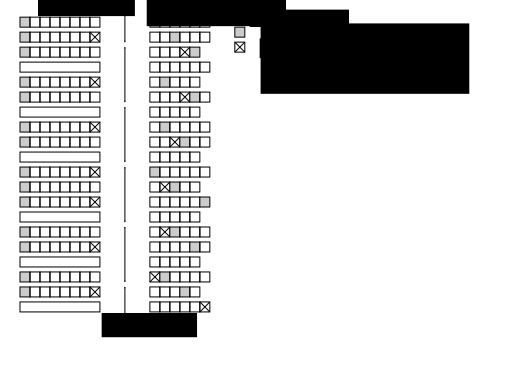
\includegraphics{./img/interrupt-period.svg.eps}
	\caption{{Sequences of packets, interrupts and PCM periods}}
	\label{fig:interrupt-period}
\end{figure}

Current implementation uses 5 milliseconds to ensure that at least one interrupt occurs between PCM periods. To apply severe latency, the interrupt interval should be changed dynamically according to sampling transmission frequency and the number of frames in a period. But this needs correct calculation and estimation for the number of packets till next PCM period.


\subsection{A lack of delay for timestamp processing}

When incoming/outgoing streams are associated and a device is a clock master, a driver uses the value of SYT field in incoming packet for the field in outgoing packet. If the master and slave handle the same value of SYT field in the same timing, the outgoing packet should include additional delay by the number of data blocks in packets in a queue. 

Current implementation simply copies the value. I have no issues about this with Fireworks/BeBoB/OXFW. To consider maintenance effort, it may be better to keep it what it is.

\subsection{A lack of PCM configuration for virtual surround nodes}

ALSA library has configuration files for each PCM component of sound card\footnote{Usually under /usr/share/alsa/cards/.}. These configuration files have settings for virtual PCM nodes. Some of these nodes are for surround channels such as "front", "side", "surround40" and so on. PulseAudio uses these nodes to decide available mapping for channels.

Such settings use "route" PCM plugin to resolve a mismatch between the number of actual channels and channels requested by ALSA PCM application. The plugin is designed to have the actual number of channels for its parameters in each configuration file.

But most of firewire devices newly supported have a different number of channels depending on models, sampling frequency and a certain modes even if they utilizes the same device chipset (Section \ref{sec:formation-data-block} to page \pageref{sec:formation-data-block}). In this reason, "route" PCM plugin is not available for the settings of these devices, while it's better to add no configuration files to ALSA library for each model because this idea requires ALSA developers to maintain 100 or more files\footnote{For example, "FWSpeakers.conf" and "FireWave.conf" were added to ALSA library 1.0.25, while they are based on OXFW970/971.}.

Instead of "route" PCM plugin, "plug" PCM plugin is available for this purpose. The plugin needs no parameters for actual channels. The plugin can resolve the mismatch of channels, as long as ALSA PCM applications open PCM nodes without "SND\_PCM\_NO\_AUTO\_CHANNELS" flag.

Unfortunately, PulseAudio uses the flag. PulseAudio fails all of trials to detect channel mapping, therefore it cannot handle the devices\footnote{[pulseaudio-discuss] 'Failed to find a working profile' for firewire sound devices http://lists.freedesktop.org/archives/pulseaudio-discuss/2014-January/019685.html}.

Furthermore, most of these firewire devices have settings for DSP (Section \ref{sec:internal-mixing}). ALSA PCM functionality can cause silence when the settings is wrong. For example, there is a device which receives AMDTP packets with 10 MBLA data channels and an ALSA application uses it as a device with stereo channels. Even if ALSA PCM functionality correctly push PCM samples into the first two data channels and fill zero PCM samples in the rest of data channels, the device can generate no sound or sound in unexpected audio ports according to the settings.

As a result, the variety of data channel make it difficult to unified configuration files, and DSP settings weaken a practical meaning of the configuration. In these reasons, current ALSA library has no configuration files for the firewire devices newly supported.

\subsection{A lack of throttles for MIDI messages in outgoing stream}
In MIDI specification, its physical layer can transfer 31,250 bit per second. This equals to 3,906 Byte per second. But in IEC 61883-6\cite{iec61883-6-1, iec61883-6-2} and MMA/AMEI RP-027\cite{amei-rp27}, AMDTP stream can transfer MIDI messages by one eighth of sampling transmit frequency (STF). This is really much than MIDI specification, therefore devices must buffer the gap between these data rate.

\begin{table}[H]
	\centering
	\caption{{Data rate for MIDI message over IEEE 1394 bus}}
	\label{tbl:midi-rate}
	\begin{tabular}{cc} \toprule
		STF	& Byte per second \\ \midrule
		32,000	& 4,000.0	\\
		44,100	& 5,512.5	\\
		48,000	& 6,000.0	\\
		88,200	& 11,025.0	\\
		96,000	& 12,000.0	\\
		176,400	& 22,050.0	\\
		192,000	& 24,000.0	\\ \bottomrule
	\end{tabular}
\end{table}

A few devices have buffer-over-flow when receiving much MIDI messages. For example, M-Audio Firewire 1814 transfer discontinuous packets when receiving much MIDI messages. There are some devices which ignores MIDI messages in more than first 8 data blocks in a packet and this seems to be a solution for this issue in vendor side.

In this reason, ALSA Firewire stack should have a throttle for MIDI messages in outgoing stream.

\subsection{A lack of control elements for ALSA control interface}

Firewire sound devices needs software implementation to control their DSP behaviour (section \ref{sec:internal-mixing} to page \pageref{sec:internal-mixing}) or device specific features.

The most devices have some ports for audio input and output. Additionally, they can receive some MBLA data channels (section \ref{sec:internal-mixing} to page \pageref{sec:internal-mixing}). Each input from audio ports and MBLA data channels can be multiplexed to each port to audio output. Furthermore, the ratio to multiplex each input to each output is changeable. As a result, this multiplexing functionality has routing settings by the number of available inputs multiplied by the number of available outputs. In FFADO, this feature is called as 'matrix mixer'.

Moreover, some devices have its specific features; phantom powering or hardware metering. The way to control these feature depends on models.

ALSA firewire drivers basically have no ALSA control interface elements because this functionality can be implemented in user-land as FFADO does. Moreover, a few devices have write-only controls, hence there is a need of permanent storage. Current ALSA control interface has no mechanism for the storage.

Currently, ffado-dbus-server/ffado-mixer is one of recommendations for this purpose but they are isolated from ALSA applications. There is an issue for transparency to ALSA applications again.

Like ALSA PCM interface, ALSA control interface has External Control plugins. It may be possible to give ways to control DSP for ALSA applications with the plugin.

A control element for the matrix mixer requires 4 parameters; sink ID, source ID, ratio. For this purpose, 'byte' type of ALSA control interface element is better with a certain structure. The plugin should inform the number of sinks/sources and the range of ratio to ALSA control applications.

If it is OK to use no control elements via control interface, it is better to implement this functionality in alsa-tools package, like envy24 or HDSP. 

Anyway, further investigation and discussion are needed for this issue.


\subsection{A lack of packet sorting}
Some Fireworks based devices sometimes transfer packets with disorder, see Figure \ref{fireworks-disorder}. Such sequence of packet is detected as discontinuity and firewire-lib stop streaming.

I've already posted my solution for this issue\footnote{[alsa-devel] [PATCH 09/39] firewire-lib: Add sort function for transmitted packet http://mailman.alsa-project.org/pipermail/alsa-devel/2014-March/073875.html} but this is rejected by a maintainer due to three points:
\begin{itemize}
\item AMDTP is nearly real-time protocol, thus it's not acceptable to have a delay of processing packets.
\item The solution apply general way to sort, while this quirk is currently confirmed only on Fireworks, thus no need to apply general way.
\item A certain pattern is confirmed to the discontinue sequence of packets. It's possible to add a few codes just for this quirk.
\end{itemize}

\begin{figure}[htbp]
\small
\begin{verbatim}
Index   Payload CIP header 1    CIP header2
032     002     3F110028        90FFFFFF
033     210     3F110030        900410E8
034     210     3F110038        900424E8
035     210     3F110040        900438E8
036     002     3F110040        90FFFFFF
037     210     3F110050 <-     900464E8
038     210     3F110048 <-     900450E8
039     210     3F110058        900478E8
040     002     3F110058        90FFFFFF
041     210     3F110068 <-     9004A4E8
042     210     3F110060 <-     900490E8
043     210     3F110070        9004B8E8
044     002     3F110070        90FFFFFF
045     210     3F110080 <-     9004E4E7
046     210     3F110078 <-     9004D0E8
\end{verbatim}
\caption{A sample of packets with disorder transmitted by Fireworks}
\label{fireworks-disorder}
\end{figure}

I confirm the disorder occurs less times than correct order. Further investigation is needed for better solution.

\subsection{A few devices freeze when frequent establishing/breaking connections}
'PreSonus FP10' can freeze when frequent establishing/breaking connections. This brings a disadvantage to PulseAudio. When PulseAudio detects the card, it starts/stops 4 streams at least. Currently PulseAudio cannot detect devices with non-surround channels. But when making PulseAudio detects the device with dbus rule and PulseAudio profiles, it may take the device freezing.

\subsection{Various results at bus reset}
Various results are confirmed with Fireworks/BeBoB at bus reset. They are depending on cases:
\begin{description}
\item{Case 1. Software bus reset} \mbox{} \\
When generating bus reset with ffado-test or jujuutils\footnote{https://code.google.com/p/jujuutils/}, streaming stopped suddenly. When generating bus reset, the drivers update connections according to IEC 61883-1. But after a few hundred millisecond, the device break connections by itself. I don't know the reason exactly but I guess the synchronizing mechanism I described has some relations.
\item{Case 2. Connecting devices or removing devices on the bus} \mbox{} \\
This case depends on which devices are connected or removed. If they are Fireworks/BeBoB based devices, streaming sometimes continues and sometimes stops. If they are not Fireworks/BeBoB based device, streaming continues. I don't know the reason exactly but I guess the synchronizing mechanism I describe have some relations. 
\end{description}

\subsection{A lack of synchronizing several devices on the same bus}
As long as reading manual of PreSonus/Focusrite/PrismSound for BeBoB based devices, there is a way to synchronize devices on the same bus. This mechanism is based on clock recovery, therefore it's driven by handling the value of SYT field in CIP packets:
\begin{itemize}
\item Driver selects a device as 'Sample clock source' then the other devices are 'Sample clock destination'.
\item Driver handles packets from the source device.
\item Driver reads SYT and calculate presentation timestamp for each devices, then transfer packets to the destination devices.
\item Driver sets recovered clock as sampling clock source for the destinations, in advance.
\end{itemize}

IEC 61883-6:2005\cite{iec61883-6-2}describes actual examples in Annex D.1.3 Embedded sample-clock jitter.

Currently ALSA Firewire stack doesn't support this mechanism. The reason is a bad balance between actual cost to implement its requirements and actual advantage to implement them. The requirements are:
\begin{itemize}
\item Requirement to manage states of several devices simultaneously
\item Requirement to handle several streams from/to all devices simultaneously
\end{itemize}

Instead of this type of synchronization, ALSA Firewire stack handle packets from a device and read SYT, then transfer packets with the value to the device. I believe this is enough for general use cases.

\newpage

\begin{thebibliography}{99}

\addcontentsline{toc}{section}{References}

\bibitem{ieee1394-1}
IEEE 1394-1995 IEEE Standard for a High Performance Serial Bus
\bibitem{ieee1394-1-a}
IEEE 1394a-2000 IEEE Standard for a High Performance Serial Bus - Amendment 1
\bibitem{ieee1394-1-b}
IEEE 1394b-2002 IEEE Standard for a High Performance Serial Bus - Amendment 2
\bibitem{ieee1394-1-c}
IEEE 1394c-2006 IEEE Standard for a High Performance Serial Bus - Amendment 3
\bibitem{ieee1394-2}
IEEE 1394-2008 IEEE Standard for a High Performance Serial Bus

\bibitem{ieee1212-1}
IEEE 1212-1991: IEEE Standard Control and Status Register (CSR) Architecture for Microcomputer Buses
\bibitem{iso13213}
ISO/IEC 13213:1994 Information technology -- Microprocessor systems -- Control and Status Registers (CSR) Architecture for microcomputer buses
\bibitem{ieee1212-2}
IEEE 1212-2001: IEEE Standard Control and Status Register (CSR) Architecture for Microcomputer Buses

\bibitem{amdtp-1}
TA Document 1997001 Audio and Music Data Transmission Protocol Version 1.0
\bibitem{amdtp-1-1}
TA Document 1999014 Enhancement to Audio and Music Transmission Protocol Version 1.0 (July 10, 2000, 1394TA)
\bibitem{amdtp-2}
TA Document 2001003 Audio and Music Data Transmission Protocol 2.0
\bibitem{amdtp-2-1}
TA Document 2001024 Audio and Music Data Transmission Protocol 2.1 (May 24, 2002, 1394TA)

\bibitem{amei-rp27}
MMA/AMEI RP-027 MIDI Media Adaptation Layer for IEEE-1394 Version 1.0 (Nov 30 2000)

\bibitem{iec61883-1-1}
IEC 61883-1:1998 Consumer audio/video equipment - Digital interface - Part 1: General, Edition 1.0
\bibitem{iec61883-1-2}
IEC 61883-1:2003 Consumer audio/video equipment - Digital interface - Part 1: General, Edition 2.0
\bibitem{iec61883-1-3}
IEC 61883-1:2008 Consumer audio/video equipment - Digital interface - Part 1: General, Edition 3.0

\bibitem{iec61883-6-1}
IEC 61883-6:2002 Consumer audio/video equipment - Digital interface - Part 6: Audio and Music Data Transmission Protocol, Edition 1.0
\bibitem{iec61883-6-2}
IEC 61883-6:2005 Consumer audio/video equipment - Digital interface - Part 6: Audio and Music Data Transmission Protocol, Edition 2.0

\bibitem{ohci1394-1}
1394 Open Host Controller Interface Specification Release 1.0 (Oct 20 1997)
\bibitem{ohci1394-1-1}
1394 Open Host Controller Interface Specification Release 1.1 (Jan 06 2000)

\bibitem{avc-general-4-2}
TA Document 2004006, AV/C Digital Interface Command Set General Specification Version 4.2 (September 1, 2004, 1394TA)
\bibitem{avc-audio-1}
TA Document 1999008, AV/C Audio Subunit 1.0 (August 21, 2000, 1394TA)
\bibitem{avc-connection-1}
TA Document 2002010, AV/C Connection and Compatibility Management Specification 1.1
\bibitem{avc-music-1}
TA Document 2001007, AV/C Music Subunit 1.0 (April 8, 2001, 1394TA)
\bibitem{avc-descriptor-1}
TA Document 1999025, AV/C Descriptor Mechanism Specification Version 1.0 (July 23, 2001, 1394TA)
\bibitem{avc-info-block-1}
TA Document 1999045, AV/C Information Block Types Specification Version 1.0 (July 23, 2001, 1394TA)
\bibitem{avc-general-enhancement}
TA Document 2000004, Enhancements to the AV/C General Specification 3.0 Version 1.1 (Oct 24, 2000, 1394TA)
\bibitem{avc-stream-format-1}
AV/C Stream Format Information Specification V1.0
\bibitem{avc-stream-format-1-1}
TA Document 2004008, AV/C Stream Format Information Specification 1.1 (working draft) (April 15, 2005, 1394TA)
\bibitem{avc-rate-control}
TA Document 1999015, AV/C Command Set for Rate Control of Isochronous Data Flow 1.0

\bibitem{icelynx}
Using TSB43Cx43A: S/PDIF Over 1394 (Dec 2003, Texas Instruments Incorrporated)
\bibitem{bebob-1}
Additional AVC commands - AV/C Unit and Subunit - SDD Products Draft 1.7-00 (Nov 17 2003, BridgeCo)
\bibitem{bebob-2}
AV/C Connection Management - Implementation Recommendation - SDD Products Draft 4.0-01 (Jul 16 2004, BridgeCo AG)

\bibitem{alsa-lib}
ALSA Library API \\
http://www.alsa-project.org/main/index.php/ALSA\_Library\_API
\bibitem{alsa-driver}
Writing an ALSA Driver (2005, Takashi Iwai) \\
http://www.alsa-project.org/main/index.php/ALSA\_Driver\_Documentation

\end{thebibliography}

\newpage

\appendix

\addcontentsline{toc}{section}{Appendices}
\addtocontents{toc}{\protect\setcounter{tocdepth}{-1}}

\section{Functions of Linux firewire subsystem}

ALSA firewire stack utilize functions exported by Linux firewire stack. In this appendix, I describe the functions.

\subsection{Serial Bus Management}

\begin{verbatim}
void fw_iso_resource_manage(struct fw_card *card, int generation,
                            u64 channels_mask, int *channel,
                            int *bandwidth, bool allocate);
\end{verbatim}

This function allocates or deallocates a channel and/or bandwidth for resources of isochronous communication by transactions to CSR\_CHANNELS\_AVAILABLE and CSR\_BANDWIDTH\_AVAILABLE in Isochronous Resource Manager.

\begin{verbatim}
void fw_schedule_bus_reset(struct fw_card *card, bool delayed,
                           bool short_reset);
\end{verbatim}

This function schedules bus reset on OHCI 1394 controller.

\subsection{Firewire subsystem transaction services}

\begin{verbatim}
typedef void (*fw_address_callback_t)(struct fw_card *card,
                                      struct fw_request *request,
                                      int tcode, int destination, int source,
                                      int generation,
                                      unsigned long long offset,
                                      void *data, size_t length,
                                      void *callback_data);
struct fw_address_handler {
        u64 offset;
        u64 length;
        fw_address_callback_t address_callback;
        void *callback_data;
        struct list_head link;
};
struct fw_address_region {
        u64 start;
        u64 end;
};
int fw_core_add_address_handler(struct fw_address_handler *handler,
                                const struct fw_address_region *region);
void fw_core_remove_address_handler(struct fw_address_handler *handler);
\end{verbatim}

The 'fw\_core\_add\_address\_handler' allocates an address region to the handler. If the address space is not already allocated or the address space is for FCP, the allocation is success. The callback in the handler is called when receiving transactions to the address space.

\begin{verbatim}
void fw_send_response(struct fw_card *card,
                      struct fw_request *request, int rcode);
int fw_cancel_transaction(struct fw_card *card,
                          struct fw_transaction *transaction);
\end{verbatim}

The 'fw\_send\_response()' and 'fw\_cancel\_transaction()' are used in the callback of the handler to send response or cancel the transaction.

\begin{verbatim}
int fw_run_transaction(struct fw_card *card, int tcode, int destination_id,
                       int generation, int speed, unsigned long long offset,
                       void *payload, size_t length);
\end{verbatim}

The 'fw\_run\_transaction()' is used to send asynchronous transaction to the node.

\subsection{OHCI 1394 isochronous contexts}

\begin{verbatim}
struct fw_iso_buffer {
        enum dma_data_direction direction;
        struct page **pages;
        int page_count;
        int page_count_mapped;
};
int fw_iso_buffer_init(struct fw_iso_buffer *buffer, struct fw_card *card,
                       int page_count, enum dma_data_direction direction);
void fw_iso_buffer_destroy(struct fw_iso_buffer *buffer, struct fw_card *card);
\end{verbatim}

This structure describes DMA mapped pages for OHCI 1394 isochronous context. The payload of each IEEE 1394 isochronous packet is stored in this buffer. 

\begin{verbatim}
struct fw_iso_context *fw_iso_context_create(struct fw_card *card,
                        int type, int channel, int speed, size_t header_size,
                        fw_iso_callback_t callback, void *callback_data);
\end{verbatim}

This function keeps isochronous context on OHCI 1394 host controller, then allocate DMA buffers for OHCI 1394 packet descriptor and IEEE 1394 isochronous packet header. The caller must allocate channel and bandwidth in advance.

\begin{verbatim}
struct fw_iso_packet {
        u16 payload_length;
        u32 interrupt:1;
        u32 skip:1;
        u32 tag:2;
        u32 sy:4;
        u32 header_length:8;
        u32 header[0];
};
\end{verbatim}

This structure basically represents IEEE 1394 Isochronous Packet. An 'interrupt' member is to generate from hardware interrupt of OHCI 1394. If the value of 'interrupt' member is 1 in every 16 packets, it means that the hardware interrupt is generated every 16 packets handled by OHCI 1394 controller.

\begin{verbatim}
int fw_iso_context_queue(struct fw_iso_context *ctx,
                         struct fw_iso_packet *packet,
                         struct fw_iso_buffer *buffer,
                         unsigned long payload);
\end{verbatim}

This function queueing given a packet to isochronous context with the buffer. The members of 'struct fw\_iso\_packet' are copied to DMA buffer for OHCI 1394 descriptor.

\begin{verbatim}
void fw_iso_context_queue_flush(struct fw_iso_context *ctx);
\end{verbatim}

This function wakes up isochronous context with queued packets.

\begin{verbatim}
int fw_iso_context_flush_completions(struct fw_iso_context *ctx);
\end{verbatim}

This function generates software interrupt (tasklet) for isochronous context.

\begin{verbatim}
int fw_iso_context_start(struct fw_iso_context *ctx,
                         int cycle, int sync, int tags);
\end{verbatim}

This function takes isochronous context to start.

\begin{verbatim}
int fw_iso_context_stop(struct fw_iso_context *ctx);
\end{verbatim}

This function takes isochronous context to stop and disable software interrupt (tasklet).

\begin{verbatim}
void fw_iso_context_destroy(struct fw_iso_context *ctx);
\end{verbatim}

This function takes isochronous context to stop and disable software interrupt, then release isochronous context and deallocate buffer.

\newpage

\section{Functions of ALSA firewire stack}

In this appendix, I describe functions of ALSA firewire stack in detail.

\subsection{Continuous packets helper functions}

These functions are in sound/firewire/iso-packets.\{c,h\}.

\begin{verbatim}
struct iso_packets_buffer {
        struct fw_iso_buffer iso_buffer;
        struct {
                void *buffer;
                unsigned int offset;
        } *packets;
};
int iso_packets_buffer_init(struct iso_packets_buffer *b, struct fw_unit *unit,
                            unsigned int count, unsigned int packet_size,
                            enum dma_data_direction direction);
void iso_packets_buffer_destroy(struct iso_packets_buffer *b,
                                struct fw_unit *unit);
\end{verbatim}

This structure includes 'struct fw\_iso\_buffer' and non-tag structure. The non-tag structure consists of pointer and offset to access the content of memory pages in packet unit. The 'iso\_packets\_buffer\_init()' function calculates the number of memory page frames with 'packet\_size' argument, 'count' argument, L1\_CACHE\_ALIGN() and PAGE\_SIZE, then keeps the pages for DMA with 'fw\_iso\_buffer\_init()'. The 'iso\_packets\_buffer\_destroy()' releases the structure.

\subsection{Isochronous Resource Management helper functions}

These functions are in sound/firewire/iso-resources.\{c,h\}.

\begin{verbatim}
struct fw_iso_resources {
        u64 channels_mask;
        struct fw_unit *unit;
        struct mutex mutex;
        unsigned int channel;
        unsigned int bandwidth;
        unsigned int bandwidth_overhead;
        int generation;
        bool allocated;
};
int fw_iso_resources_init(struct fw_iso_resources *r,
                          struct fw_unit *unit);
void fw_iso_resources_destroy(struct fw_iso_resources *r);
int fw_iso_resources_allocate(struct fw_iso_resources *r,
                              unsigned int max_payload_bytes, int speed);
int fw_iso_resources_update(struct fw_iso_resources *r);
void fw_iso_resources_free(struct fw_iso_resources *r);
\end{verbatim}

The structure 'fw\_iso\_resources' represents an manager for isochronous resource such like channel and bandwidth. The 'fw\_iso\_resources\_init()' initializes it and 'fw\_iso\_resources\_destroy()' release it.
The 'fw\_iso\_resources\_allocate()' keeps isochronous resources with given 'max\_payload\_bytes' and 'speed'. The 'fw\_iso\_resources\_update()' reallocate isochronous resources to handle bus reset. The 'fw\_iso\_resources\_free()' releases isochronous resources. Most operations utilizes 'fw\_iso\_resource\_manage()' in Linux firewire subsystem.

\subsection{CMP helper functions}

These functions are written in sound/firewire/cmp.\{c,h\}.

\begin{verbatim}
enum cmp_direction {
        CMP_INPUT = 0,
        CMP_OUTPUT,
};
struct cmp_connection {
        int speed;
        bool connected;
        struct mutex mutex;
        struct fw_iso_resources resources;
        __be32 last_pcr_value;
        unsigned int pcr_index;
        unsigned int max_speed;
        enum cmp_direction direction;
};
int cmp_connection_init(struct cmp_connection *connection,
                        struct fw_unit *unit,
                        enum cmp_direction direction,
                        unsigned int pcr_index);
int cmp_connection_check_used(struct cmp_connection *connection, bool *used);
void cmp_connection_destroy(struct cmp_connection *connection);
int cmp_connection_establish(struct cmp_connection *connection,
                             unsigned int max_payload);
int cmp_connection_update(struct cmp_connection *connection);
void cmp_connection_break(struct cmp_connection *connection);
\end{verbatim}

The 'struct cmp\_connection' includes parameters related to CMP such like PCR index. The 'cmp\_connection\_init()' check Output/Input MPR by a READ transaction according to given 'direction' and 'pcr\_index', then initialize 'resources' member. The 'cmp\_connection\_destroy()' release these structures. The 'cmp\_connection\_establish()' keeps isochronous resources and establishes a connection by a LOCK transaction. The 'cmp\_connection\_update()' updates a connection by a LOCK transaction to handle bus reset. The 'cmp\_connection\_break()' breaks an established connection by a LOCK transaction. The connection should be broken before destroyed.

The 'cmp\_connection\_check\_used()' is a bit special. This is added for relationships to drivers in user-space. When the drivers handle devices, the caller of this function can check the driver's connection.

\subsection{AMDTP stream helper functions}

These functions are in sound/firewire/amdtp.\{c,h\}.

\begin{verbatim}
enum amdtp_stream_direction {
        AMDTP_OUT_STREAM = 0,
        AMDTP_IN_STREAM
};
enum cip_flags {
        CIP_NONBLOCKING         = 0x00,
        CIP_BLOCKING            = 0x01,
        CIP_SYNC_TO_DEVICE      = 0x02,
        CIP_EMPTY_WITH_TAG0     = 0x04,
        CIP_DBC_IS_END_EVENT    = 0x08,
        CIP_WRONG_DBS           = 0x10,
        CIP_SKIP_DBC_ZERO_CHECK = 0x20,
        CIP_SKIP_INIT_DBC_CHECK = 0x40,
        CIP_EMPTY_HAS_WRONG_DBC = 0x80,
};
struct amdtp_stream {
        struct fw_unit *unit;
        enum cip_flags flags;
        enum amdtp_stream_direction direction;
        struct fw_iso_context *context;
        struct mutex mutex;

        struct iso_packets_buffer buffer;
        int packet_index;

        enum cip_sfc sfc;
        unsigned int syt_interval;

        unsigned int source_node_id_field;
        unsigned int data_block_quadlets;
        unsigned int data_block_counter;
        unsigned int pcm_channels;
        unsigned int midi_ports;
        u8 pcm_positions[AMDTP_MAX_CHANNELS_FOR_PCM];
        u8 midi_position;

        unsigned int tx_dbc_interval;

        unsigned int transfer_delay;
        unsigned int data_block_state;
        unsigned int last_syt_offset;
        unsigned int syt_offset_state;

        struct amdtp_stream *sync_slave;

        bool callbacked;
        wait_queue_head_t callback_wait;

        struct snd_pcm_substream *pcm;
        void (*transfer_samples)(struct amdtp_stream *s,
                                 struct snd_pcm_substream *pcm,
                                 __be32 *buffer, unsigned int frames);
        unsigned int pcm_buffer_pointer;
        unsigned int pcm_period_pointer;
        bool pointer_flush;
        struct tasklet_struct period_tasklet;

        struct snd_rawmidi_substream *midi[AMDTP_MAX_CHANNELS_FOR_MIDI * 8];
        unsigned int rx_blocks_for_midi;
};
\end{verbatim}

This structure represents an AMDTP stream. Currently this structure is for AM824 data. An AMDTP stream can transfer one PCM substream and 8 MIDI substreams. The 'buffer' member is for continuous packet buffer, and the 'index' member is for handling the continuous packets. The 'sfc' and 'syt\_interval' are dominant parameters. These parameters are decided by stream's nominal sampling rate:

\begin{verbatim}
enum cip_sfc {
        CIP_SFC_32000  = 0,
        CIP_SFC_44100  = 1,
        CIP_SFC_48000  = 2,
        CIP_SFC_88200  = 3,
        CIP_SFC_96000  = 4,
        CIP_SFC_176400 = 5,
        CIP_SFC_192000 = 6,
        CIP_SFC_COUNT
};
extern const unsigned int amdtp_syt_intervals[CIP_SFC_COUNT] = {
        [CIP_SFC_32000]  =  8,
        [CIP_SFC_44100]  =  8,
        [CIP_SFC_48000]  =  8,
        [CIP_SFC_88200]  = 16,
        [CIP_SFC_96000]  = 16,
        [CIP_SFC_176400] = 32,
        [CIP_SFC_192000] = 32,
};
\end{verbatim}


The 'source\_node\_id\_field', 'data\_block\_quadlets', 'data\_block\_counter' are for CIP header. The 'tx\_dbc\_interval' is for a device-specific quirk which has fixed interval for the value of data block counter, not compliant to IEC 61883-1.

The 'transfer\_delay', 'data\_block\_state', 'last\_syt\_offset', 'syt\_offset\_state' are used to generate the value of SYT field in non-blocking mode without timestamp synchronization. The 'sync\_slave' is used for blocking mode with duplex streams with timestamp synchronization to handle timestamps in incoming packets to outgoing packets.

The 'callbacked' and 'callback\_wait' are used to wait till a first packet is available.

The 'pcm' and 'transfer\_samples' members are used to multiplex/demultiplex PCM samples into an AMDTP packet. The 'pcm\_buffer\_pointer', 'pcm\_period\_pointer', 'pointer\_flush', 'period\_tasklet' are used to call 'snd\_pcm\_period\_elapsed()' in period boundary.

The 'midi' member is used to multiplex/demultiplex MIDI message into an AMDTP packet. The 'rx\_blocks\_for\_midi' is for a model-specific quirk to ignore MIDI messages in data blocks more than a certain numbers in a packet.

\begin{verbatim}
bool cip_sfc_is_base_44100(enum cip_sfc sfc);
\end{verbatim}

The 'cip\_sfc\_is\_base\_44100()' returns given 'sfc' is 44100, 88200, 176400 or not.

\begin{verbatim}
int amdtp_stream_init(struct amdtp_stream *s, struct fw_unit *unit,
                      enum amdtp_stream_direction dir,
                      enum cip_flags flags);
\end{verbatim}

The 'amdtp\_stream\_init()' initializes members in the structure. This function gets reference counter from given 'struct fw\_unit'. The 'dir' and 'flags' are important for an AMDTP stream.

\begin{verbatim}
void amdtp_stream_destroy(struct amdtp_stream *s);
\end{verbatim}

The 'amdtp\_stream\_destroy()' clear some members in the structure. This function put reference counter to given 'struct fw\_unit'. The caller is sure to stop the stream in advance.

\begin{verbatim}
void amdtp_stream_set_parameters(struct amdtp_stream *s,
                                 unsigned int rate,
                                 unsigned int pcm_channels,
                                 unsigned int midi_ports);
\end{verbatim}

The 'amdtp\_stream\_set\_parameters()' sets parameters to given stream structure. As a result, the stream structure has values in 'sfc', 'syt\_interval', 'pcm\_channels', 'midi\_ports', 'data\_block\_quadlets', 'transfer\_delay' fields. This function also initializes 'pcm\_positions' and 'midi\_positions' according to IEC 61883-6:2005.

\begin{verbatim}
unsigned int amdtp_stream_get_max_payload(struct amdtp_stream *s);
\end{verbatim}

The 'amdtp\_stream\_get\_max\_payload()' returns the number of bytes as maximum size of payload of CIP for an AMDTP packet. The caller must call 'amdtp\_stream\_set\_parameters()' in advance.

\begin{verbatim}
void amdtp_stream_set_sync(enum cip_flags sync_mode,
                           struct amdtp_stream *master,
                           struct amdtp_stream *slave);
\end{verbatim}

As a default, the synchronization mode is simplex stream without timestamp synchronization. The 'amdtp\_stream\_set\_sync()' set synchronization mode between master and slave streams for duplex streams with timestamp synchronization.

\begin{verbatim}
int amdtp_stream_start(struct amdtp_stream *s, int channel, int speed);
bool amdtp_stream_wait_callback(struct amdtp_stream *s, unsigned int timeout);
\end{verbatim}

The 'amdtp\_stream\_start()' starts an amdtp stream over given channel and speed. Then Linux Firewire subsystem start isochronous context and to handle related interrupts. The 'amdtp\_stream\_wait\_callback()' is to wait till a first packet can be available or timeout with given value.

\begin{verbatim}
bool amdtp_stream_running(struct amdtp_stream *s);
bool amdtp_streaming_error(struct amdtp_stream *s);
\end{verbatim}

The 'amdtp\_stream\_running()' is to check whether the stream is running or not. The 'amdtp\_streaming\_error()' is to check whether the stream is stopped with errors. The reasons of error is described later in this chapter.

\begin{verbatim}
void amdtp_stream_update(struct amdtp_stream *s);
\end{verbatim}

The 'amdtp\_stream\_update' is used to update the 'source\_node\_id\_field' member, basically to handle bus reset. Internally, amdtp\_stream\_start() also calls this function.

\begin{verbatim}
void amdtp_stream_stop(struct amdtp_stream *s);
\end{verbatim}

The 'amdtp\_stream\_stop' stops and destroys isochronous context, to stop an AMDTP stream. Then this function releases the buffer for continuous packets.

\subsection{PCM substream helper functions for AMDTP stream}

\begin{verbatim}
#define AMDTP_IN_PCM_FORMAT_BITS        SNDRV_PCM_FMTBIT_S32
#define AMDTP_OUT_PCM_FORMAT_BITS       (SNDRV_PCM_FMTBIT_S16 | \
                                         SNDRV_PCM_FMTBIT_S32)
\end{verbatim}

These macro is for 'struct snd\_pcm\_hardware.formats'. This represents current firewire-lib capability.

\begin{verbatim}
#define AMDTP_MAX_CHANNELS_FOR_PCM      64
\end{verbatim}

This macro represents the maximum number of PCM channels which current firewire-lib can handle.

\begin{verbatim}
int amdtp_stream_add_pcm_hw_constraints(struct amdtp_stream *s,
                                        struct snd_pcm_runtime *runtime);
\end{verbatim}

This function adds constraints to given PCM substream runtime according to given stream.

\begin{verbatim}
void amdtp_stream_set_pcm_format(struct amdtp_stream *s,
                                 snd_pcm_format_t format);
\end{verbatim}

The 'amdtp\_stream\_set\_pcm\_format()' sets 'transfer\_samples' member into stream according to given format. This is expected to be called in 'struct snd\_pcm\_ops.hw\_params()'.

\begin{verbatim}
void amdtp_stream_pcm_prepare(struct amdtp_stream *s);
\end{verbatim}

The 'amdtp\_stream\_pcm\_prepare()' initializes members related to handling 'snd\_pcm\_period\_elapsed()'. This is expected to be called in 'struct snd\_pcm\_ops.prepare()'.

\begin{verbatim}
unsigned long amdtp_stream_pcm_pointer(struct amdtp_stream *s);
\end{verbatim}

The 'amdtp\_stream\_pcm\_pointer()' returns the number of frames in an PCM ring buffer.

\begin{verbatim}
void amdtp_stream_pcm_trigger(struct amdtp_stream *s,
                              struct snd_pcm_substream *pcm);
\end{verbatim}

The 'amdtp\_stream\_pcm\_trigger()' sets 'pcm' member to given AMDTP stream. This is expected to be called in 'struct snd\_pcm\_ops.trigger'.

\begin{verbatim}
void amdtp_stream_pcm_abort(struct amdtp_stream *s);
\end{verbatim}

The 'amdtp\_stream\_pcm\_abort()' stops PCM substream with XRUN state. This is expected to be used before stopping AMDTP stream.

\begin{verbatim}
bool amdtp_stream_pcm_running(struct amdtp_stream *s);
\end{verbatim}

The 'amdtp\_stream\_pcm\_running()' is to check whether PCM substreams is running on the AMDTP stream or not.


\subsection{MIDI substream helper functions for AMDTP stream}

\begin{verbatim}
#define AMDTP_MAX_CHANNELS_FOR_MIDI     1
\end{verbatim}

This describes the maximum number of MIDI Conformant data channels in an AMDTP packet which firewire-lib can handle. 8 MPX-MIDI data streams are multiplexed into one MIDI Conformant data channel\cite{amei-rp27, iec61883-6-2}, hence the number of maximum MIDI ports which firewire-lib can support is 8.

\begin{verbatim}
void amdtp_stream_midi_trigger(struct amdtp_stream *s,
                               unsigned int port,
                               struct snd_rawmidi_substream *midi)
\end{verbatim}

The 'amdtp\_stream\_midi\_trigger()' set MIDI substream to given AMDTP stream. This is expected to be called in 'struct snd\_rawmidi\_ops.trigger'.


\subsection{Transaction service helper function}

These functions are in sound/firewire/lib.\{c,h\}.

\begin{verbatim}
#define FW_GENERATION_MASK      0x00ff
#define FW_FIXED_GENERATION     0x0100
#define FW_QUIET                0x0200
int snd_fw_transaction(struct fw_unit *unit, int tcode,
                       u64 offset, void *buffer, size_t length,
                       unsigned int flags);
\end{verbatim}

This function is a helper for an asynchronous transaction. Usually this function retries three times if the transaction is failed because of error or bus\_reset. With the flag 'FW\_FIXED\_GENERATION', this function doesn't retry and returns error if bus reset occurs. The flag 'FW\_QUIET' suppress error message.

\subsection{FCP helper functions}

These functions are in sound/firewire/fcp.\{c,h\}.

\begin{verbatim}
int fcp_avc_transaction(struct fw_unit *unit,
                        const void *command, unsigned int command_size,
                        void *response, unsigned int response_size,
                        unsigned int response_match_bytes);
\end{verbatim}

The 'fcp\_avc\_transaction()' sends an AV/C command frame to the target and wait for the corresponding response frame. The 'response\_match\_bytes' is a bitmap to match frames of command/response in bytes unit. This function supports deferred transaction in AV/C General\cite{avc-general-4-2}.

\begin{verbatim}
void fcp_bus_reset(struct fw_unit *unit);
\end{verbatim}

The 'fcp\_bus\_reset()' is used to handle bus reset. All of pending AV/C transactions are terminated and retried. 


\subsection{AV/C General commands}

These functions are in sound/firewire/fcp.\{c,h\}.

\begin{verbatim}
#define AVC_PLUG_INFO_BUF_BYTES 4
enum avc_general_plug_dir {
        AVC_GENERAL_PLUG_DIR_IN         = 0,
        AVC_GENERAL_PLUG_DIR_OUT        = 1,
        AVC_GENERAL_PLUG_DIR_COUNT
};
int avc_general_get_plug_info(struct fw_unit *unit, unsigned int subunit_type,
                              unsigned int subunit_id, unsigned int subfunction,
                              u8 info[AVC_PLUG_INFO_BUF_BYTES]);
\end{verbatim}

The 'avc\_general\_plug\_dir()' is used to get plug information according to AV/C General\cite{avc-general-4-2}. Extended addressing is not supported.

\begin{verbatim}
int avc_general_set_sig_fmt(struct fw_unit *unit, unsigned int rate,
                            enum avc_general_plug_dir dir,
                            unsigned short plug);
int avc_general_get_sig_fmt(struct fw_unit *unit, unsigned int *rate,
                            enum avc_general_plug_dir dir,
                            unsigned short plug);
\end{verbatim}

The 'avc\_general\_set\_sig\_fmt()' and 'avc\_general\_get\_sig\_fmt()' are used to set/get current sampling rate according to AV/C General\cite{avc-general-4-2}. Extended addressing is not supported.

\end{document}
